\documentclass[11pt,a4paper]{report}

\usepackage{float}
\usepackage{amsmath}
\usepackage{amsfonts}
\usepackage{pdflscape}
\usepackage{longtable}
\usepackage{parskip}
\usepackage[hyphens]{url}
\usepackage[hidelinks]{hyperref}
\usepackage[margin=3.5cm]{geometry}
\usepackage{appendix}
\usepackage{graphicx}
\usepackage{subfigure}
\usepackage[font={small}]{caption}
\usepackage{multicol}
\usepackage{enumitem}

\usepackage[bottom]{footmisc}
\usepackage{longtable}

\usepackage{minted}
\usemintedstyle{manni}

\usepackage{tikz}
\usetikzlibrary{positioning,shapes,arrows,fit,calc}

\usepackage{todonotes}

% Stretch table cell height
\renewcommand{\arraystretch}{1.5}

%%%%%%%%%%%%%%%%%%%%%%%%%%%%%%%%%%%%%%%%%%%%%%%%%%%%%%%%%%%%%%%%%%%%%%%%%%%%%%%%
% BIBLATEX SETTINGS
%%%%%%%%%%%%%%%%%%%%%%%%%%%%%%%%%%%%%%%%%%%%%%%%%%%%%%%%%%%%%%%%%%%%%%%%%%%%%%%%
\usepackage[
backend=bibtex,
firstinits=true,    % Render first and middle names as initials
maxcitenames=2,     % Use maximum 2 names in \cite before et al.
maxbibnames=99,      % Use maximum 2 names in references before et al.
style=authoryear,
dashed=false,       % Re-print recurring author names in bibliography
]{biblatex}

% Use single quotes around titles:
\usepackage[british]{babel}
\usepackage{csquotes}

% Add a blank line between references
\setlength{\bibitemsep}{\baselineskip}

% Don't use reference months
\AtEveryBibitem{\clearfield{month}}
\AtEveryCitekey{\clearfield{month}}

% All author's names should be Last, First
\DeclareNameAlias{author}{last-first}

% Insert a comma between author and year in text citations
\renewcommand*{\nameyeardelim}{\addcomma\addspace}

% Remove 'in:' preceding article title
\renewbibmacro{in:}{}

\addbibresource{../bibliography.bib}

%%%%%%%%%%%%%%%%%%%%%%%%%%%%%%%%%%%%%%%%%%%%%%%%%%%%%%%%%%%%%%%%%%%%%%%%%%%%%%%%

\begin{document}

\begin{titlepage}
\center
\vspace*{3.5cm}

{\Large
    Electronics and Computer Science\\
    Faculty of Physical Sciences and Engineering\\
    University of Southampton\\[1cm]
}

{\large
    Jamie Davies\\
    \today\\[1cm]
}


{\LARGE
    A Non-Personalised Approach to\\
    Twitter Hashtag Recommendations \\[1.5cm]
}

A project report submitted for the award of\\
MEng Computer Science\\[1.5cm]

\emph{Supervisor:}\\
Dr.\ Nick Gibbins\\[0.5cm]

\emph{Examiner:}\\
Dr.\ Klaus-Peter Zauner\\


\vfill
\end{titlepage}

\pagenumbering{roman}

\begin{abstract}
\todo[noline]{Make shorter}
One of the key characteristics of Twitter and other microblogging platforms is the use of `hashtags' --- topical/categorical annotations provided by the authors of the posts (tweets) themselves. This flexible system was designed for the effective organisation and searching of tweets, but with Twitter facing an ever-increasing number of users and tweets it is hard for users to keep track of the vast number of hashtags in popular use. This results in data from the hashtags being fragmented and inaccurate due to the users making poor or uninformed hashtag choices.

If users are presented with a choice of relevant hashtags when writing a tweet, they are more likely to publish tweets with accurate tag data. This project aims to create an intelligent hashtag recommendation tool to improve the quality of the information we can gain from hashtags. However, whilst such a system could improve future tweets, tweets that have already been published will remain untouched by the system. Thus, the system will be extended to also retrofit hashtags to published tweets --- allowing for tweets to appear in search results for a particular hashtag even if they don't actually contain the hashtag in question.

\todo[inline]{Add more about scope of project}
\end{abstract}
\pagebreak

\tableofcontents

\pagebreak

\subsection*{Acknowledgements}
Thank you to everyone involved in the creation of this project. Most importantly, thank you to Nick Gibbins for providing the inspiration for this project. Thank you to Jon and Sina for giving up their time to give me the advice and enthusiasm I needed. Thanks to Katie for having the patience to be optimistic when I couldn't remember how. Thank you to Hayden and Miles, for making the \LaTeX\ styling of this document a constant competition. Thanks to Mum and Dad for their support and proofreading. Finally, thanks to everyone who downloaded and used Spout, the response to the package was overwhelming.

\subsection*{Statement of Originality}

The work contained within this report has not been previously submitted for a degree or diploma at any other higher education institution. To the best of my knowledge and belief, this project contains no material previously published or written by another person except where due references are made.

\pagebreak

\setcounter{page}{1}
\pagenumbering{arabic}

\chapter{Introduction}
\label{chap:introduction}
Collaborative tagging (sometimes referred to as social tagging) systems are designed to allow users to navigate, organise and manage online resources. The central idea behind these systems is the concept of an annotation: the action of a user applying a personalised tag to a resource. On a large scale, many of these annotations can be taken together to form a complex network of users, resources and tags --- commonly referred to as a `folksonomy' \parencite{Xu:2008}.

One of the most popular applications of a folksonomy is Twitter\footnote{\url{www.twitter.com}}. `Hashtags', which are simply any combination of letters or digits preceded by a hash character (\#), afford users the ability to create free-form tags to describe the content of their posts (`tweets'). Tweets can be categorized with several hashtags, thereby creating networks of tweets and users, and making it easy to find other related tweets, users and hashtags. This renders hashtags as a powerful tool in aiding the search and navigation of the billions of tweets contained within Twitter.

However, despite its numerous benefits, the hashtag system presents new challenges to overcome before it can become truly useful. Due to the open nature of folksonomies, it is important that users have the freedom to create and use exactly the tags they wish to use. However, this unsupervised tagging can result in vast numbers of hashtags for users to choose from, often including redundant or ambiguous hashtags. When posting a tweet, there is nothing stopping a user from creating an entirely new hashtag to describe something with exactly the same meaning as a collection of other hashtags. This redundancy can confuse users and fragment the true meaning behind the synonymous hashtags.

Evidence of this problem can be easily found through a casual navigation of popular hashtags or topics on Twitter. It is commonplace for users to use a collection of tags in one tweet that are all synonymous. An example of this can be seen from an arbitrarily chosen tweet (with the author's personal details removed) in Figure~\ref{fig:badtagging}.

\begin{figure}[htpb]
    \centering
    
\includegraphics[width=0.65\linewidth]{badtagging.png}
    \caption{An example showing the poor tagging practices used on Twitter.}
    \label{fig:badtagging}
\end{figure}

\section{Project Goals}

The goal of this project is to develop an intelligent hashtag recommendation system for use with Twitter. The objective is to make it easier for users to select appropriate meaningful hashtags for their tweets, and in doing so, begin to tackle the problems presented by the sheer quantity and redundancy of hashtags in Twitter. The aim is that the user will be able to see hashtag suggestions in real-time as they are typing a tweet, thus making them more likely to publish tweets with accurate hashtag data.

Such a recommendation system would also need to aid users in the navigational and exploratory aspects of folksonomies. Therefore, another objective for this project is to make it easier for users to navigate and search the content available on Twitter, thus making the fragmented hashtag data already published easier to search and navigate. The aim is that the same recommendation system used to suggest hashtags for content a user is creating could also be applied to create enhanced search queries to retrieve tweets from Twitter.

\pagebreak

\chapter{Background Literature \& Related Work}
\label{chap:litreview}
The motivation behind hashtags is to categorise tweets and allow them to show up more easily in searches\footnote{\url{https://support.twitter.com/articles/49309-using-hashtags-on-twitter}}. Whilst the task that this project is aiming to complete is novel and fairly unexplored, it is well connected with other experiments, systems and projects within the research community.

\section{Traditional Recommendation Systems}
Traditional recommendation systems are in place all over the web today. From music discovery services \todo{Add screenshots of existing recommendation services?}(such as Last.fm\footnote{\url{www.last.fm}}) to suggested purchases on retail sites (like on the front page of Amazon\footnote{\url{www.amazon.co.uk}}), these systems are all personalised recommendation engines that take an individual user's preferences and use them to provide suggestions tailored to that user.

Most personalised recommendation systems employ a set of techniques known as collaborative filtering. These techniques were first coined by \textcite{Goldberg:1992}, where a system named \emph{Tapestry} was created that allowed people to attach annotations to documents, and then use that information to filter the documents for other users.

One common implementation of collaborative filtering is the so-called ``user-to-user'' approach. ``User-to-user'' collaborative filtering works by taking the preferences of a user $A$, and finding a small subset of other users in the system that have similar preferences. For each user $B$ in the subset, any items that $B$ has adopted that $A$ hasn't are added to a ranked list of suggestions. $A$ is now more likely to adopt items in the list than the items of another random person \parencite{Schafer:2001}.

Another approach to provide relevant recommendations to a user is the use of content-based recommendation systems. This is a type of system that recommends items relevant to other items by comparing their details and descriptions. This can be extended to suggest items for a user by comparing a content-based description of the user's preferences with the descriptions of the items \parencite{Pazzani:2007}.

A key issue with content-based filtering is that the recommendations can only be as accurate as the algorithm used to derive a user's profile. There are a number of algorithms available to build user profiles, depending upon the context, but essentially a content-based profile is created using a weighted vector of item features. The weights mark the importance of each feature to the user, and can be computed from individually rated content vectors.

\textcite{Cantador:2010} studied and evaluated a number of content-based recommendation models based upon the premise of user and item profiles being described in terms of weighted lists and tags. Through their experiments they found that models that focused on user profiles outperformed the models oriented towards item profiles in nearly every test. They go on to suggest that a better way of profiling users would be through the use of tag clustering.

Instead of limiting recommendation systems to the accuracy of their classifiers, a common approach is to incorporate relevance feedback techniques. Relevance feedback is a process that was originally designed for information retrieval, and works on the assumption that a user can not always correctly encapsulate into a query what it is they are searching for. It works by allowing a user to create a query to which an initial set of results is returned. From these, the user can then mark certain results as relevant or irrelevant. This information is then submitted and used to refine the original query and return more relevant results to the user \parencite{Salton:1990}.

\textcite{Utiyama:2006} showed that it is possible to combine collaborative filtering, content-based filtering and relevance feedback techniques into one system to provide better recommendations.

\section{Assigning Labels with Machine Learning Techniques}
Although there exists a long history of research into traditional recommendation algorithms, the data structure of a folksonomy is distinct from those found in traditional problems. This has led to a new generation of supervised learning classification algorithms which can be applied to the problem of assigning labels to resources.

In order to facilitate the comparison of resources, tags and users, aggregate projections of the data can be constructed. This reduces the dimensionality of the data by sacrificing some information \parencite{Schmitz:2006}. There are two main classes of algorithms that perform this task: feature \emph{selection}, which reduces the size of a dataset by selecting a subset of the data, and feature \emph{extraction}, which uses the existing data to generate entirely new features. Despite the improved results that feature extraction can provide, their computational cost and memory requirements can often make them impractical for use on the extremely large datasets common with folksonomies \parencite{Gemmell:2009}.

One compromise to this trade-off is to use an algorithm such as Hebbian Deflation, which approximates the outputs of the intensive feature extraction techniques, but with lower computational cost and memory requirements \parencite{Oja:1985}. \textcite{Gemmell:2009} used this approach coupled with a \todo{Add more about K-Nearest Neighbour implementation?}$k$-Nearest Neighbour classifier to find appropriate tags for a given resource. This was done by finding `neighbouring' users: ``Neighbours are selected only if they have tagged the query resource and tags are selected for the recommendation set only if they have been applied by the neighbour to the resource'' \parencite{Gemmell:2009}. It was tested on data from the popular bookmarking site Delicious\footnote{\url{http://delicious.com/}} and from Citeulike\footnote{\url{http://www.citeulike.com/}}, a tool that enables researchers to manage and discover scholarly references, and it was found to be a successful approach with giving results.

\textcite{Niwa:2006} took a different approach to overcome the limitations of collaborative filtering. Using a modified version of the \todo{Add more TF-IDF implementation detail?}TF-IDF \parencite{Salton:1988}, they calculate the affinity level between users and tags (where affinity level is a measure of how frequently a user uses a particular tag), and then use this to calculate the similarity between tags. These similarity measures are then clustered using a custom clustering algorithm to provide a set of recommended tags for a given user and resource. This enabled them to adjust the level at which a user's preferences were taken into account when determining recommendations, as well as providing a simple solution to the tag redundancy issue found across most folksonomies.

Another popular machine learning approach to the folksonomy tag recommendation problem is the use of a Naive Bayes classifier. Naive Bayes has been an accepted tool in information retrieval for a long time, with some early literature dating back over 50 years \parencite{Maron:1960}, and has recently been seeing a renaissance within the machine learning community.

As shown by \textcite{DePessemier:2010}, Naive Bayes can be easily adapted and extended to work in the context of providing recommendations to match a query or a set of user preferences. In particular, their algorithm relies upon the general user preferences for cases where the classifier produced an uncertain outcome, and becomes more context specific on a sliding scale as the classifer gives more certain probabilities.

\section{Approaches to Hashtag Recommendation}
Even though providing hashtag recommendations and suggestions is still a new and largely unexplored field, there have been several efforts to improve the hashtag experience for Twitter users.

The current hashtag system on Twitter (Figure~\ref{fig:twittersuggest}) uses a non-personalised auto-complete tool to provide suggestions to the user. Whenever a hash symbol (\#) is typed in the tweet composer, the system suggests hashtags starting with the letters that the user has typed so far. These suggestions are chosen from a tiny subset of hashtags, taken from a mixture of those currently trending\footnote{Trending hashtags are those with the highest rise in usage within a given time period.} and from the user's history. Whilst better than not having suggestions at all, this system is only truly useful in one of two specific use cases: when the user knows the starting letters of a trending hashtag they want to use, or are trying to recall a hashtag that they have previously used. This system does not help the user choose the correct hashtag for the content of their tweet.

\begin{figure}[htpb]
    \centering
    
\includegraphics[width=0.5\textwidth]{twittersuggest.png}
    \caption{Twitter's current hashtag suggestion system.\label{fig:twittersuggest}}
\end{figure}

By assuming that the primary purpose of hashtags is to categorise tweets and improve searching (as Twitter envisioned), \textcite{Zangerle:2011} created a system that recommends hashtags for a tweet by taking hashtags from other tweets that are textually similar to the query. The similarity between tweets is calculated with the TF-IDF model. The hashtags are then extracted from the similar tweets, ranked according to their similarity to the original query, and returned as a list of suggestions to the user. A number of different ranking algorithms were tested, but this was found to be the most successful.

After studying the advantages of providing personalised recommendations in retail situations on a per-user basis, \textcite{Kywe:2012} realised that a similar approach towards hashtags could prove fruitful. Hashtag use varies from user to user, with some users using the latest trending hashtags, other users only using a specific set or type of tag, and with some users barely using them at all. They proposed a personalised hashtag recommendation system that considers both user preferences and the query tweet content: the system creates a ranked list of hashtags from both the most similar users and most similar tweets. This gave promising results, although it was noted that this may not be the best recommendation system for all types of tweets and hashtags.

\textcite{Shepitsen:2008} used a hierarchical agglomerative clustering algorithm to profile users and provide personalised recommendations in collaborative tagging systems. They found that clusters of tags can be effectively used to ascertain a user's interests, which could then be used in a traditional content-based recommendation approach. This technique worked well, particularly for dense folksonomies such as Last.fm.

Observers of social media have realised that hashtags play a dual role within the online microblogging communities, such as Twitter. On one hand, hashtags fulfil the design goals that Twitter created them to accomplish (bookmarking and improving search); on the other hand, however, they serve as a badge of community membership: connecting users together. \textcite{Yang:2012} took this duality into account when attempting to create a hashtag recommendation system by training a support vector machine (SVM) classifier with a variety of features taken from the tweet metadata to overcome the duality and suggest relevant hashtags.

\pagebreak

\chapter{Analysis}
\label{chap:analysis}

\section{Preliminary Data Analysis}

To investigate the usage of hashtags and the problems associated with them further, a dataset of 500,000 tweets was collected from the sample Twitter stream over a time period of approximately 4.5 days. The tweets collected were filtered to ensure that they were in English, and contained at least one hashtag.

Through the use of some trivial Python scripts, it is easy to find evidence of poor hashtag choices. In particular, the most overwhelming observation is the quantity of redundant hashtags in use throughout Twitter. Table~\ref{tbl:redundancy} shows several hashtags taken from the dataset and their number of occurrences. Despite the tags all having exactly the same semantic meaning, the use of the tags is fragmented.

\begin{table}[htpb]
\centering
\begin{tabular}{| l | l |}
    \hline
    \textbf{Hashtag} & \textbf{Number of Occurrences} \\
    \hline \hline
    \#peopleschoice & 94849 \\ \hline
    \#peopieschoice & 2043 \\ \hline
    \#peoplechoice  & 439 \\ \hline
    \#peoplesch     & 287 \\ \hline
    \#peopleschoi   & 269 \\ \hline
    \#peoplesc      & 230 \\ \hline
    \#peoplescho    & 219 \\ \hline
    \#peolpeschoice & 164 \\ \hline
    \#peopleschioce & 137 \\ \hline
    \#pca           & 94 \\ \hline
\end{tabular}
\caption{Occurrences of hashtags referring to the People's Choice Awards}
\label{tbl:redundancy}
\end{table}

Another interesting observation is that of the times that different hashtags are used, which varies greatly from hashtag to hashtag. Some tags are used in tweets at a fairly uniform rate (Fig.~\ref{fig:android}), whilst others feature large spikes of usage over a short period of time (Fig.~\ref{fig:blackfriday}). This demonstrates the communities behind the hashtags --- rather than a hashtag being used at a particular time for a particular event, some hashtags are used consistently by users to join in on a large-scale conversation.

\begin{figure}[htpb]
    \centering
    \subfigure[\#android]{
        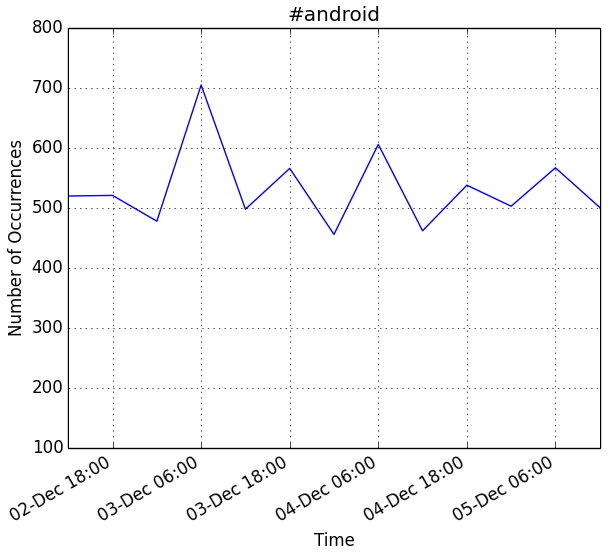
\includegraphics[width=0.45\textwidth]{android}
        \label{fig:android}
    }
    \subfigure[\#blackfriday]{
        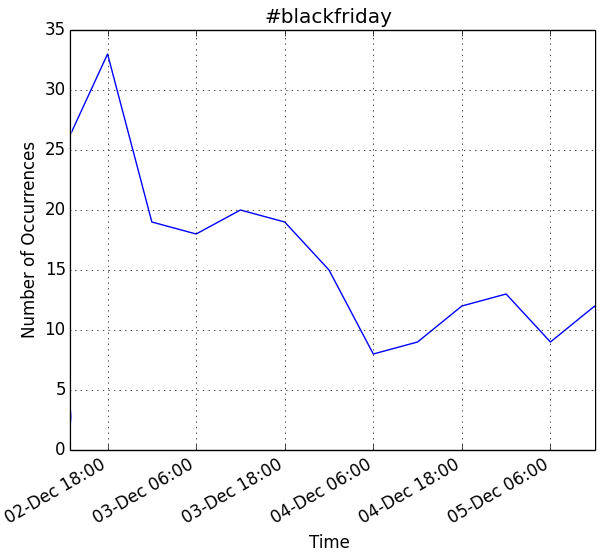
\includegraphics[width=0.45\textwidth]{blackfriday}
        \label{fig:blackfriday}
    }
    \caption{Usage of hashtags over the period that the dataset was collected.}
\end{figure}

\section{Requirements}

As demonstrated above, there is a need for a hashtag recommendation system to improve the quality and clarity of hashtags in Twitter, as well as to aid navigation of the already existing fragmented data. This leads to the two main requirements the system in this project must fulfil:
\begin{itemize}
    \item Users should be able to compose and publish tweets whilst the system suggests hashtags relevant to the content of their tweets.
    \item Users should be able to search for a hashtag and view related tweets, including those that don't contain that hashtag.
\end{itemize}

As seen from the research and discussion presented in Chapter~\ref{chap:litreview}, most existing approaches to providing recommendations within a folksonomy make extensive use of user preferences in their algorithms. From calculating a `neighbourhood' of similar users to falling back on a set of users' preferences when the data is unclear, most current approaches provide a personalised recommendation system.

This raises the question of whether hashtags are clearly defined, or whether their meanings (and therefore the tweets they apply to) are dependent upon user opinion. Through the preliminary examination of a sample Twitter dataset conducted in Chapter~\ref{chap:introduction}, this project is inclined to believe that the correct usage of a hashtag is independent of how frequently a particular user uses that hashtag. Indeed, it could be argued that a user's preference towards a particular hashtag can result in incorrect hashtags being used --- which is the very problem this project is aiming to tackle.

This indicates another requirement of the recommendation system:
\begin{itemize}
    \item The system must provide identical recommendations for all users, user preferences should not be taken into account.
\end{itemize}

As with all folksonomies, there is not a predefined set of hashtags available to users on Twitter, meaning new hashtags are created and used every day. With this in mind it becomes clear that a lot of data will be needed to train the recommendation system, so that it successfully recognises and recommends a sufficient number of hashtags. This gives another requirement of the system:
\begin{itemize}
    \item The system must be capable of training on a sufficiently large dataset of tweets, with potential to use the live data from the Twitter stream.
\end{itemize}

Lastly, Twitter is available through its web platform on practically every internet-connected device that exists today. For this system to be successfully implemented and used by Twitter users, it too must be available on all of Twitters supported devices. In addition to this, it must be as easy to post a tweet using the recommendation system as it is on Twitter.
\begin{itemize}
    \item The system must be accessible through a web interface that provides quick and easy access to the recommendation system.
\end{itemize}

From these broad requirements, a complete set of formal requirements can be inferred:

\subsection{Functional Requirements}
\label{ssec:funcreqs}
\begin{enumerate}
    \item \label{func:publish} The system must allow the user to log in and publish tweets using their Twitter account.
    \item \label{func:suggest} The system must provide hashtag recommendations as the user is writing a tweet.
    \item \label{func:search} The system must perform a hashtag search through a large dataset of tweets and return all relevant tweets, including those that do not contain the search query.
    \item \label{func:genmodel} The system must use information from a large dataset of tweets to generate a model representing each hashtag.
    \item \label{func:notpersonal} The system must only use the data available through the Twitter API, and not make use of any other externally collected metrics, such as user preferences.
    \item \label{func:compmodels} The system must be able to compare tweets against its representational hashtag models.
    \item \label{func:stream} \emph{Optional:} In place of a large dataset, the system could be able to use information from the live Twitter stream.
    \item \label{func:probabilities} \emph{Optional:} The system could provide probabilities for how likely a hashtag is to be related to a tweet.
\end{enumerate}

\subsection{Non-Functional Requirements}
\label{ssec:nfuncreqs}
\begin{enumerate}
    \item \label{nfunc:web} The system must be accessible via a web interface.
    \item \label{nfunc:easy} The system must be responsive and easy to use.
    \item \label{nfunc:qsearch} The system must be able to perform searches quickly.
    \item \label{nfunc:qsuggest} The system must be able to make hashtag recommendations quickly.
    \item \label{nfunc:graphs} \emph{Optional:} The system could be able to produce visualisations to provide an easy way to interpret the hashtag recommendations/assignments.
    \item \label{nfunc:mobile} \emph{Optional:} The system could be accessible via mobile web browsers.
\end{enumerate}

\pagebreak

\chapter{Design}
\label{chap:design}

\section{Architecture}

The primary aim of the system is to produce an ordered list of recommended hashtags for a given string with a maximum length of 140 characters (a tweet). The secondary aim is to facilitate query expansion when searching Twitter for a hashtag. Due to non-functional requirement~\ref{nfunc:web}, both of these sub-systems must be available through a web interface. It is unreasonable and infeasible to expect all necessary training and classification to occur in code running within the user's browser, especially considering that some of those browsers might be on low-powered mobile platforms. For these reasons, a client-server architecture has been chosen for the system.

Using a client-server software model will allow for a distinct separation between the hashtag recommendation system and any interfaces that make use of the tool. The server (Figure~\ref{fig:serveroverview}) will be running a single instance of the recommendation engine, and will handle all training and classification events. Multiple clients (Figure~\ref{fig:clientoverview}) can then query the classifier running on the server for either hashtag suggestions or a search query expansion.

\begin{figure}[htpb]
    \centering
    \subfigure{
        \begin{tikzpicture}
            \node[rectangle,draw,text width=5cm,anchor=north,rectangle split, rectangle split parts=2,text justified] (server) {
                \textbf{Server}
                \nodepart{second}- Hashtag recommendation\newline
                - Search query expansion\newline
                - Training classifier\newline
                - Persistent state
            };
        \end{tikzpicture}
        \label{fig:serveroverview}
    }
    \subfigure{
        \begin{tikzpicture}
            \node[rectangle,draw,text width=5cm,anchor=north,rectangle split, rectangle split parts=2,text justified] (client) {
                \textbf{Client}
                \nodepart{second}- Twitter authentication\newline
                - Twitter API calls\newline
                - Send requests to server\newline
                - Receive data from server
            };
        \end{tikzpicture}
        \label{fig:clientoverview}
    }
    \caption{Functional overviews of the server and client.}
\end{figure}

This design ensures that there is a very light load on the clients using the tool, which is an ideal solution to enabling usage of the system from all internet-connected devices (non-functional requirements \ref{nfunc:web} and \ref{nfunc:mobile}).

Another benefit of using a centralised server to encapsulate the hashtag recommendation system is the clear separation of functionality between the client and server. This means that the interface that the user sees and interacts with is distinct from the technical functionality --- enabling multiple differently styled interfaces to connect to the recommendation server. It even presents the possibility of one day integrating with the Twitter web platform itself.

\section{Abstract Implementation}

When using a client-server execution model, it is important to correctly balance the tasks that need to be executed between the clients, the server and the users. Placing a high computational load on the users' machines can limit the accessibility of the system, whilst placing a high computational load on the server can cause a slow-down or even interrupted service for all clients using the system.

The server encapsulates the hashtag classifier system. It will have the ability to train the classifier on tweet data independently and asynchronously to the other tasks that the classifier may need to perform. The training will perform as many of the computationally intensive operations on the classifier model as it feasibly can, to ensure that any requests from a client to classify a tweet or expand a query are performed as quickly as possible (fulfilling non-functional requirements \ref{nfunc:qsearch} and \ref{nfunc:qsuggest}). Asynchronous training will also provide the opportunity to integrate training data from the live Twitter stream (as described in functional requirement~\ref{func:stream}).

The client's primary focus will be delivering the interface to the users. It will provide a way for the user to interact with the recommendations and search tools available on the server, as well as handling the users' authentication with Twitter and calling appropriate tweet or search functions in the Twitter API.

\begin{figure}[htpb]
    \centering
    \begin{tikzpicture}[
        node distance=7mm,
        title/.style={anchor=west,font=\fontsize{9}{9}\color{black}\ttfamily},
        typetag/.style={rectangle, draw=black!50, anchor=west}
    ]
        % Server
        \node (server) [title] {Server};
            \node (classifier) at ($(server.west)+(0,-28pt)$) [title,xshift=2mm] {Classifier};
                \node (worker) at ($(classifier.west)+(0,-28pt)$) [title,xshift=2mm] {Worker Process};
                    \node (train) [below=of worker.west,typetag] {Training Function};
                \node (swebserver) at ($(train.west)+(0,-32pt)$) [title] {Web Server};
                    \node (recommend) [below=of swebserver.west,typetag] {Hashtag Recommendation};
                    \node (query) [below=of recommend.west,typetag] {Search Query Expansion};

        \node (workerbox) [draw,fit={(worker) (train)}] {};
        \node (swebserverbox) [draw,fit={(swebserver) (recommend) (query)}] {};
        \node (classifierbox) [draw,fit={(classifier) (workerbox) (swebserverbox)}] {};
        \node (serverbox) [draw,fit={(server) (classifierbox)},line width=1.5pt] {};


        % Client
        \node (client) at (7.5cm, 0) [title] {Client};
        \node (cwebserver) at ($(client.west)+(0,-28pt)$) [title,xshift=2mm] {Web Server};
                \node (auth) [below=of cwebserver.west,typetag] {Twitter Authentication};
                \node (api) [below=of auth.west,typetag] {Twitter API Calls};
                \node (interface) [below=of api.west, typetag] {Interface};

        \node (cwebserverbox) [draw,fit={(cwebserver) (auth) (api) (interface)}] {};
        \node (clientbox) [draw,fit={(client) (cwebserverbox)},line width=1.5pt] {};


        % Users
        \node (a) at (8.3cm, -5.3cm) [draw,circle,minimum width=1cm] {User};
        \node (b) at (9.8cm, -5.3cm) [draw,circle,minimum width=1cm] {User};
        \node (c) at (11.3cm, -5.3cm) [draw,circle,minimum width=1cm] {User};


        % Twitter
        \node (twitter) at (6.4cm, 2.5cm) [cloud,draw,cloud puffs=10,cloud puff arc=120,aspect=2,inner ysep=1em] {Twitter};


        % Arrows
        \draw[<->] (a) -- (interface);
        \draw[<->] (b) -- (interface);
        \draw[<->] (c) -- (interface);
        \path[<->] (clientbox) edge node[sloped, anchor=center, above] {\footnotesize HTTP} (swebserverbox);
        \draw[<->] (clientbox) -- (twitter);
        \draw[->,dashed] (twitter) -- (train);
    \end{tikzpicture}
    \caption{An abstract view of the implementation of the system.}
    \label{fig:abstractdetail}
\end{figure}

\section{Classification Algorithm}
To choose an appropriate classification algorithm, two main factors were considered. One factor was that the classifier had to be capable of being trained incrementally. This is so that the classifier can be trained upon a stream, and simultaneously still provide valid classifications. This is essential, as some classifiers require parsing the entire data set before they are able to provide classifications, making them unsuitable for working with data stream. The other factor to consider was that of probabilities: it was decided that it would be suitable for the classifier to return the probabilities of the hashtag recommendations it suggests (as seen in functional requirement~\ref{func:probabilities}).

These considerations led to the choice of a Naive Bayes classifier. Naive Bayes is built upon Bayes' Theorem, which explains how to derive the probability of an event happening given that another event has occurred:

\begin{equation}
    P(A|B) = \frac{P(B|A) \cdot P(A)}{P(B)}
\end{equation}

This can be expanded to give the probability of a classification based upon the presence of a set of features by making a \textbf{naive assumption}: that the presence of a particular feature is totally unrelated and unaffected by the presence (or lack) of any other feature. By making this assumption, we can derive the probabilistic model for a Naive Bayes classifier:

\begin{equation}
    P(C|F_1,\dots,F_n) = \frac{P(F_1,\dots,F_n)|C) \cdot P(C)}{P(F_1,\cdots,F_n)}
\end{equation}

Or, in plain English terminology:

\begin{equation}
    P(\text{Hashtag}|\text{Features}) = \frac{P(\text{Features}|\text{Hashtag}) \cdot P(\text{Hashtag})}{P(\text{Features})}
\end{equation}

\section{Data Features}
As seen in the equations above, to predict hashtags for a tweet it is necessary to transform that tweet into a set of features. There are a number of approaches to this, and not all are limited to the text of the tweet. For instance, it could be possible to extract features from other information that is available with each tweet, such as date and time, or the location that the tweet was posted from. However, these are continuous variables and therefore present the extra challenge of discretisation before they can be used in a Naive Bayes classifier.

To reduce complexity the feature extraction in this project will be based solely upon the actual text that makes up the tweets themselves.

\section{User Interface}
\label{sec:wireframes}
Whilst the primary focus of this project is the creation of the tool to provide hashtag suggestions and query expansions (the server), a prototype interface will also be developed. This interface will enable users to log in to Twitter, post tweets using hashtag suggestions, and search Twitter using query expansion.

Figure~\ref{fig:wireframe:tweet} shows the design of the interface for creating a tweet. It follows conventional HCI principles, including displaying the site name and navigation in the top left, and having the user's username and user-oriented controls in the top right. There is a single box for the user to type their tweet message into, and as they are typing into this box, relevant hashtag suggestions will appear underneath. Clicking on one of these hashtags will insert it at the end of the text in the box.

Figure~\ref{fig:wireframe:searchresults} shows the design of the interface for searching Twitter. It follows the same HCI guidelines as most other search results pages, and keeps the same layout as the tweet composition page (and indeed, all other pages in the client interface).

\begin{figure}[htpb]
    \centering
    \subfigure[Tweet composition page.]{
        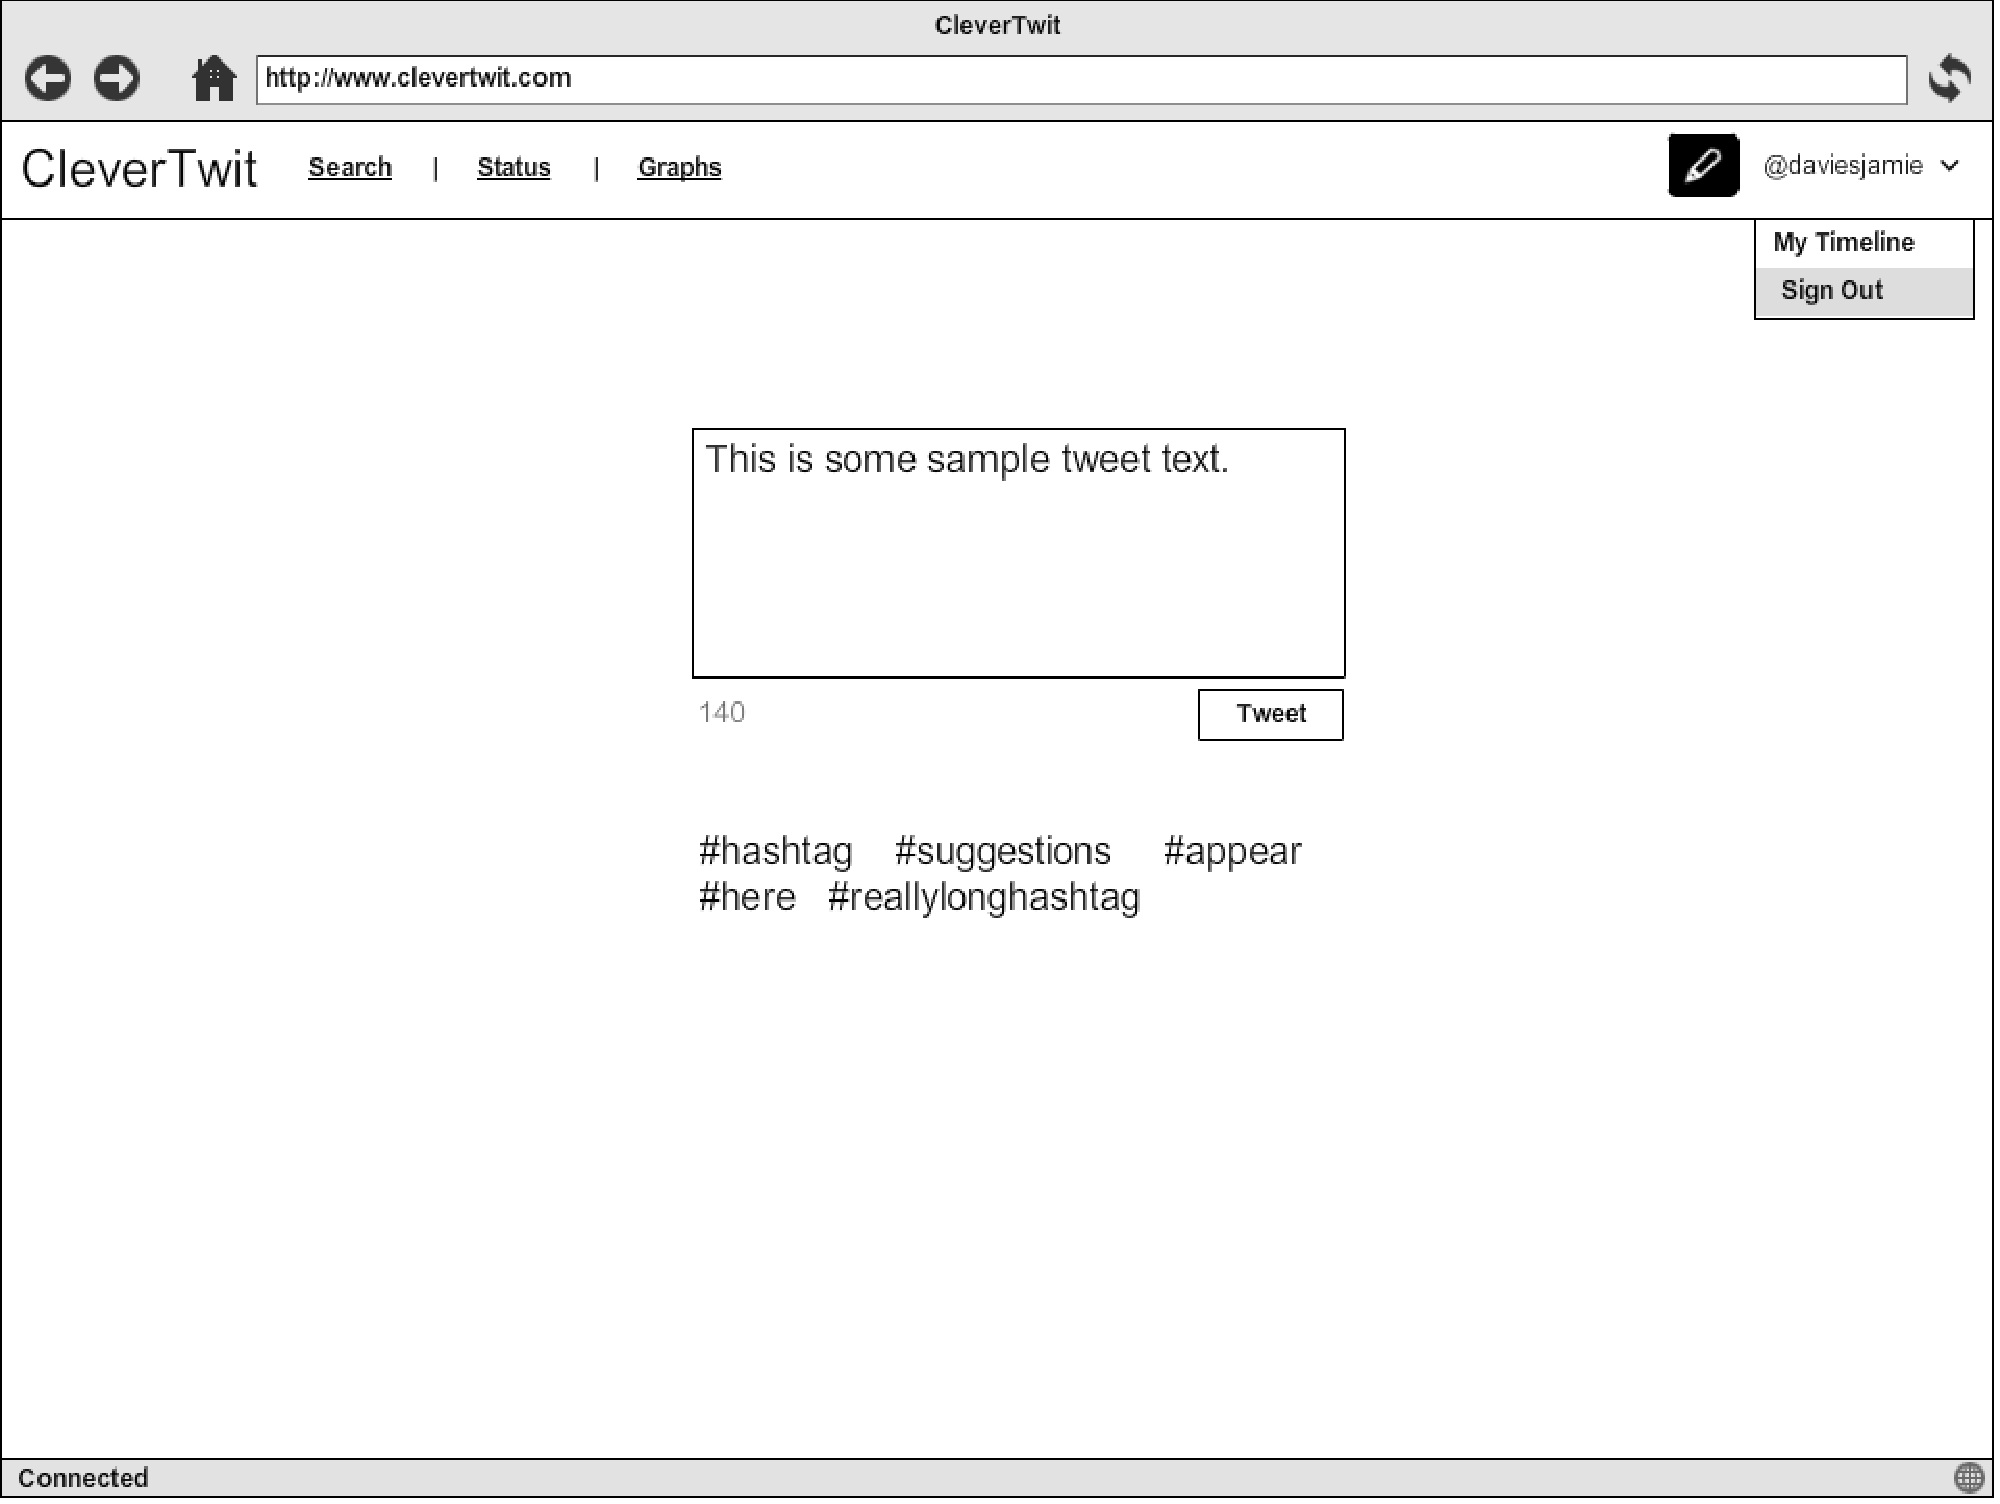
\includegraphics[width=0.9\linewidth]{wireframes/tweet.pdf}
        \label{fig:wireframe:tweet}
    }
%    \subfigure[The beginning search page.]{
%        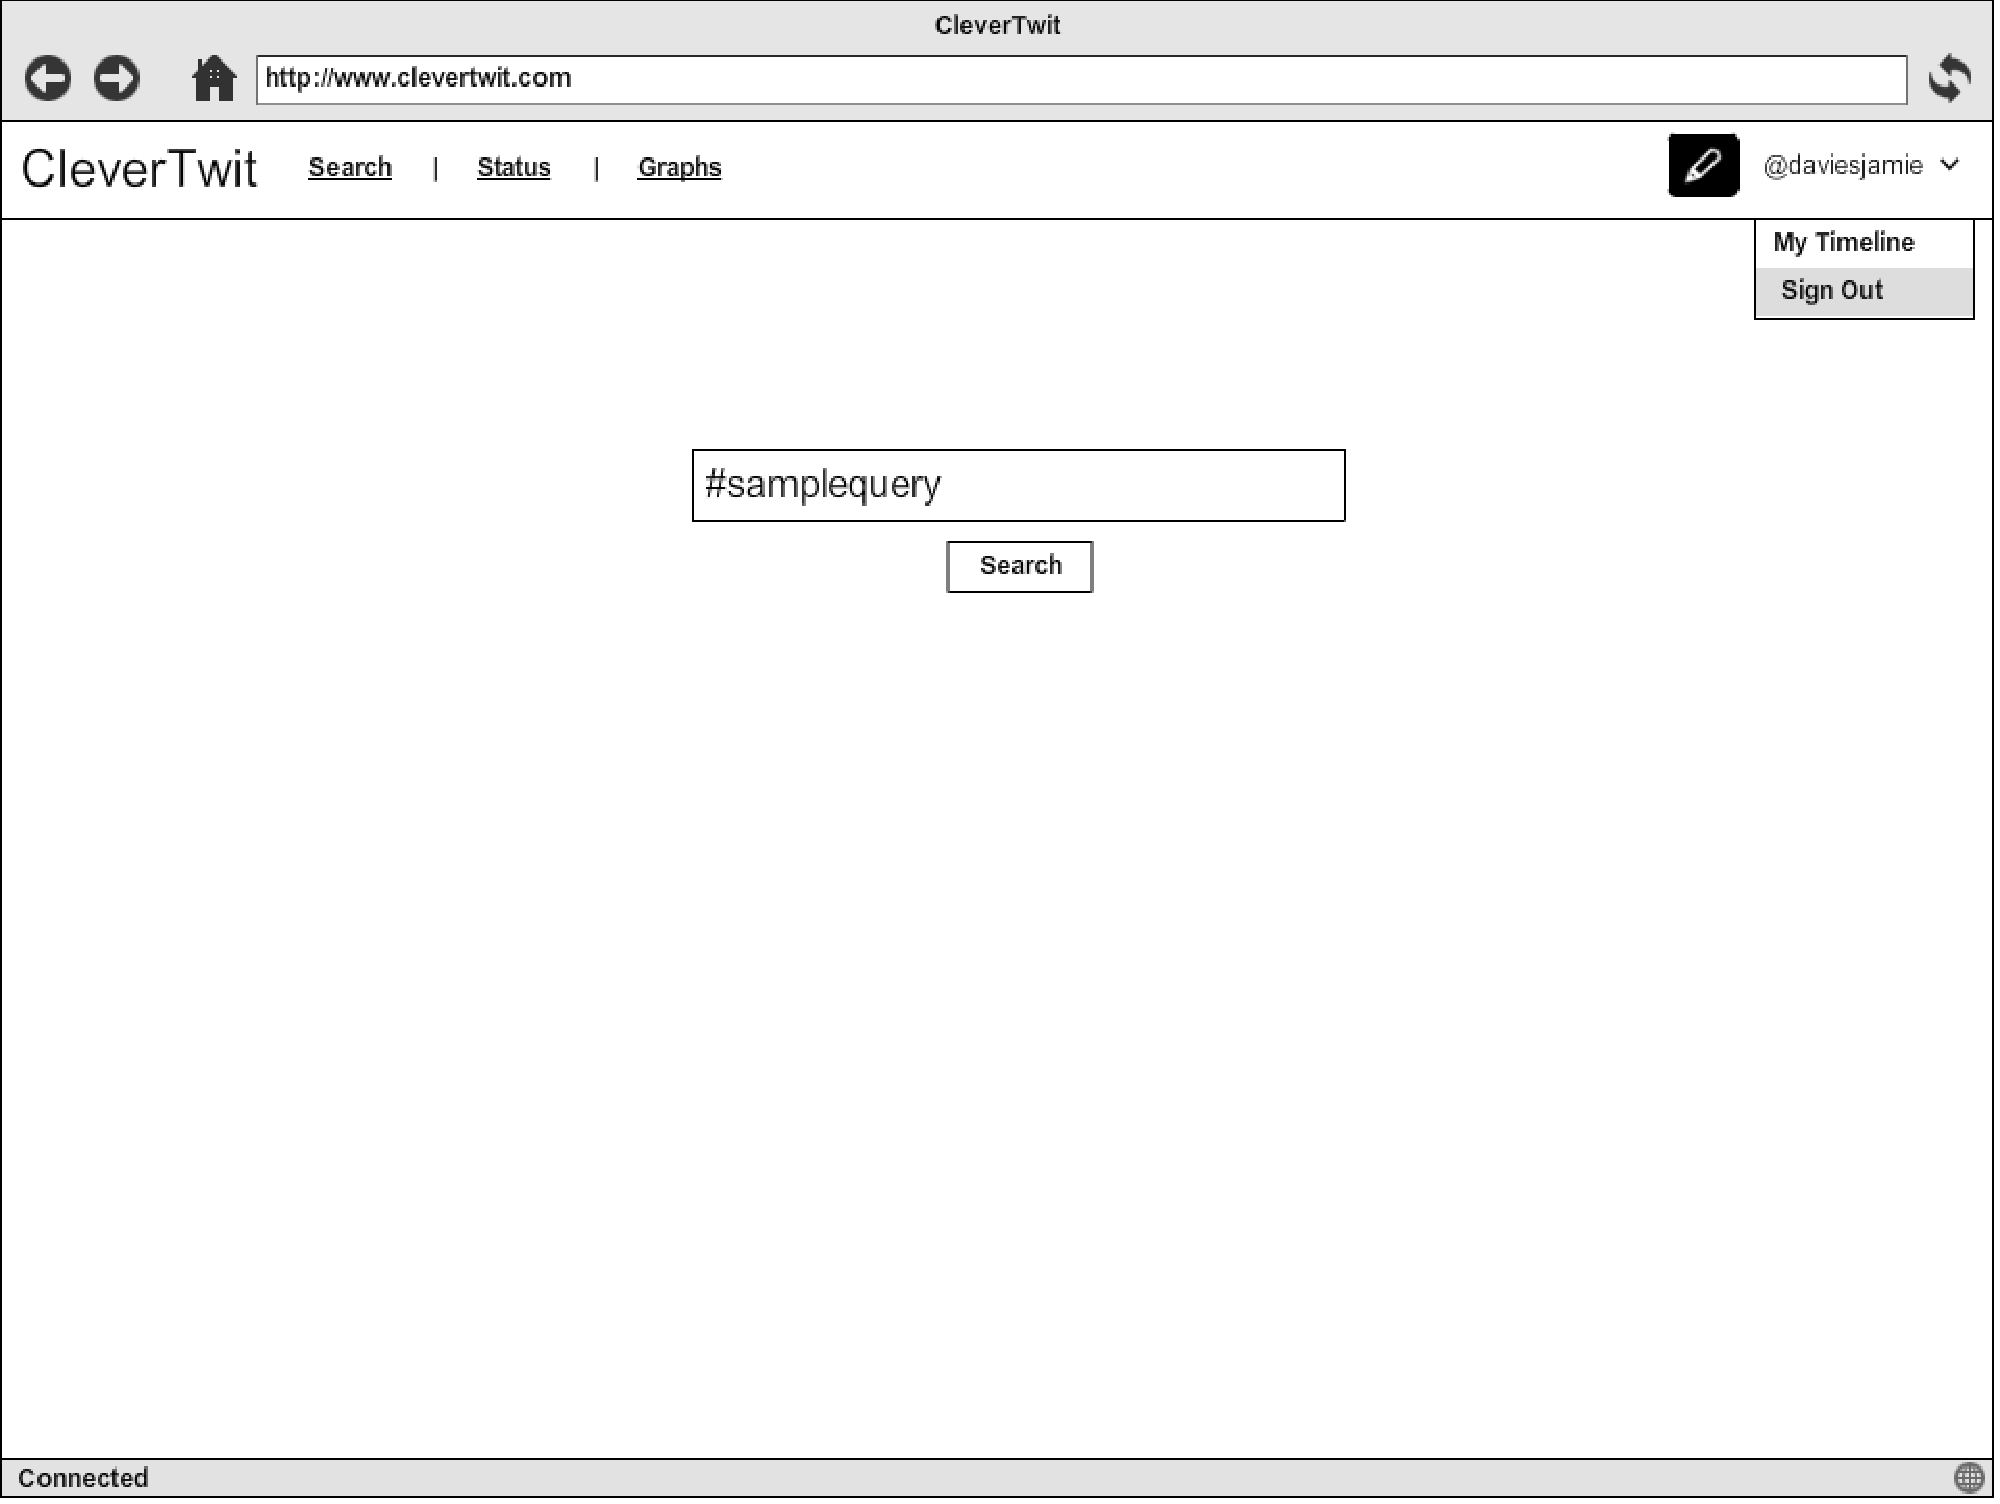
\includegraphics[width=0.8\linewidth]{wireframes/search.pdf}
%        \label{fig:wireframe:search}
%    }
    \subfigure[The search results page.]{
        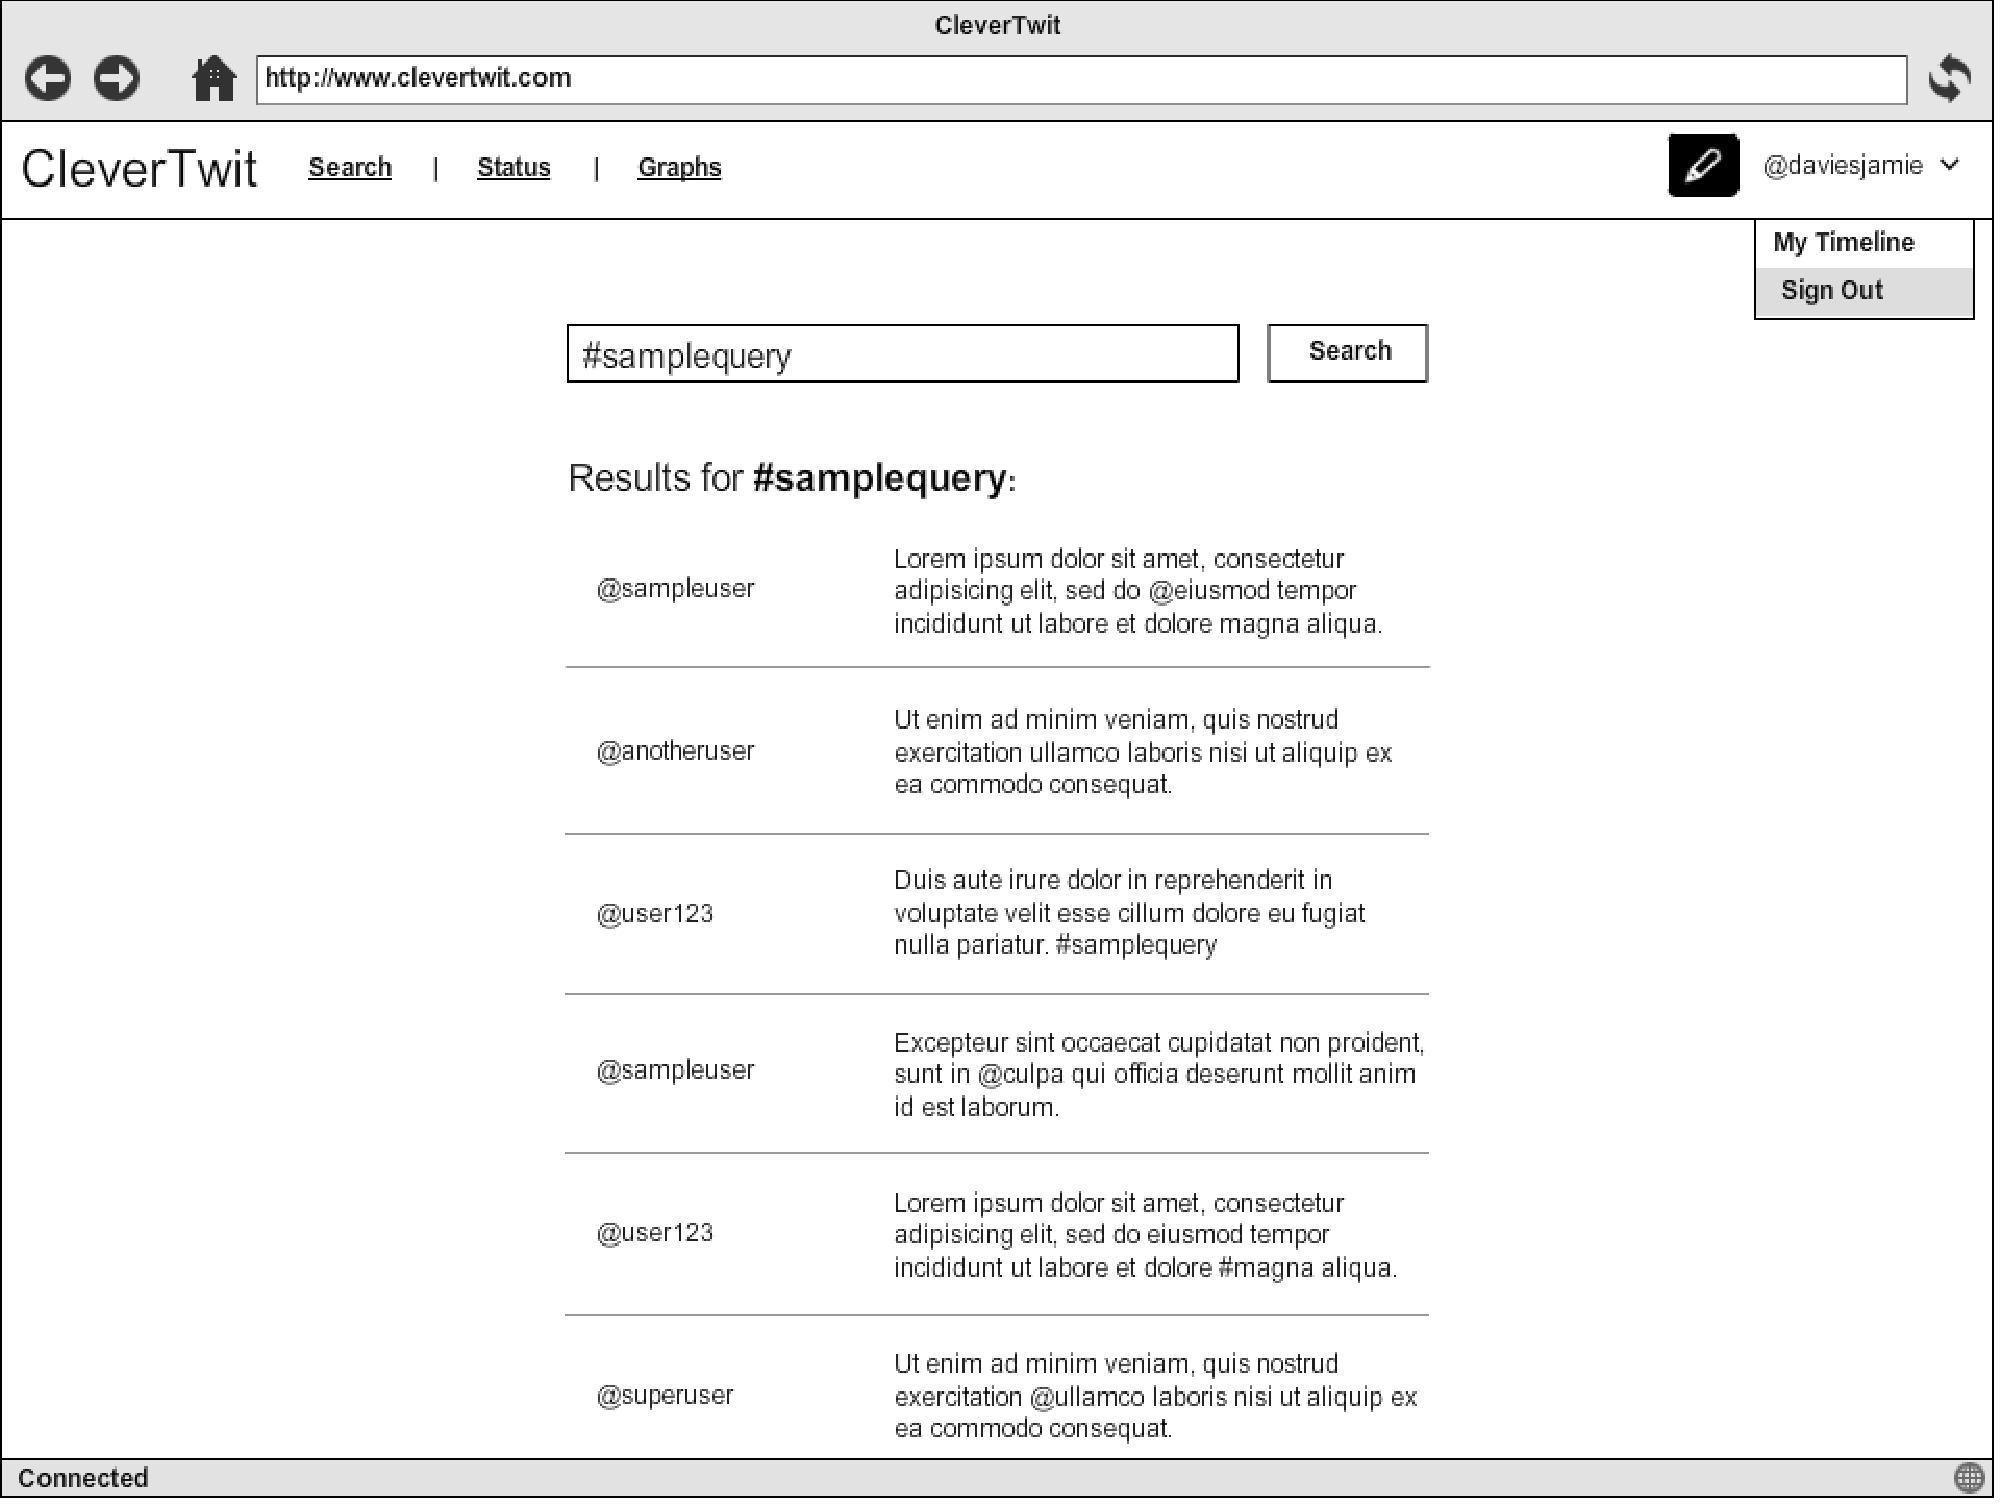
\includegraphics[width=0.9\linewidth]{wireframes/searchresults.pdf}
        \label{fig:wireframe:searchresults}
    }
    \caption{Wireframe designs of the prototype interface.}
    \label{fig:wireframes}
\end{figure}

\pagebreak

\chapter{Implementation}
\label{chap:implementation}

This chapter explains how the system was implemented, and the decisions that were made during the process. It also shows any difficulties that were encountered, and how they were dealt with.

\section{Tools \& Technologies}
The first decision to make when implementing the system was to decide upon the programming languages, technologies and libraries that would be used.

Python 2.7 was chosen as the language of choice for the majority of the project, including both the server and the content management system for the client. Python is a widely used high-level programming language whose syntax emphasises code readability and maintainability. Most importantly, it has a strong developer community behind it, resulting in a large collection of excellent third-party libraries, including the following:

\begin{description}
    \item[Django\footnotemark]\footnotetext{\url{www.djangoproject.com}} offers a simple and flexible way of following the traditional MVC (Model-View-Controller) programming paradigm. This made it easy to develop the client system, by providing a structured way to keep the authentication and page generation separate from the layout and design of the page. Django also offers a pleasant interface to handling web requests.
    \item[Flask\footnotemark]\footnotetext{\url{http://flask.pocoo.org}} and \textbf{Tornado\footnote{\url{www.tornadoweb.org}}} are a web application frameworks made with Python, that make it simple to create efficient and scalable web APIs and WSGI applications. They are used to create and handle the HTTP endpoints for the server.
    \item[Twython\footnotemark]\footnotetext{\url{http://github.com/ryanmcgrath/twython}}, a thin but functional Python wrapper around the Twitter API, makes API calls easily available within Python. It also provides a set of methods that handle authentication with Twitter.
\end{description}

Python 3 was not chosen for the project as it is still in its infancy. Many existing libraries written for Python have not yet been adapted for Python 3, and most operating systems or installers default to Python 2.7. To be successful, the system in this project has to be as easy to integrate and set up as possible --- and therefore Python 2.7 was chosen.

The client interface itself was written with a combination of HTML, CSS and Javascript. In particular, the following tools and libraries were used:

\begin{description}
    \item[Twitter Bootstrap\footnotemark]\footnotetext{\url{http://getbootstrap.com}}, a front-end framework that enables sleek and interactive interfaces with minimal customisation, allowing for easier and faster web development. It also has the bonus of being the UI toolkit that Twitter itself uses, and gives the client interface a look and feel similar to that of Twitter. Lastly, Bootstrap makes use of CSS3 to provide a full responsive interface, allowing the same web page to be viewed across all devices, regardless of the screen size --- which helps to fulfil non-functional requirement \ref{nfunc:mobile}.
    \item[JQuery\footnotemark]\footnotetext{\url{www.jquery.com}}, a Javascript library that contains a huge set of predefined functions and classes. It is designed to simplify client-side Javascript, and makes it much easier to manipulate the document object model (DOM) from within Javascript --- it is used specifically within the client to perform asynchronous Javascript and XML requests (AJAX requests) to the server, and provide live hashtag suggestions.
\end{description}

\section{Spout: A Data Stream Processing Framework}
\label{sec:spout}
To give the possibility of using either the live Twitter stream or a static file of tweets as the data source for the classifier, it was decided that the input data should be operated on as a stream. Doing so would allow identical processing of the tweet data, regardless of where the data came from.

Taking inspiration from a section of OpenIMAJ \parencite{Hare:2011}, a library with a fluent interface was created to enable such a processing paradigm. A fluent interface is the use of chaining method calls together to relay the instruction context of a subsequent call, to improve the readability of the code. At the heart of the library is the concept of a stream, which is simply a sequential (and not necessarily finite) collection of data items. The \verb+Stream+ class defines the basic operations that can be performed upon a data stream:

\begin{description}
    \item[Mapping] \hfill \\
        The items in one stream can be mapped to another stream. This is done by applying a supplied \verb+Function+ object to each item in the input stream, to produce another output stream.
        \mint{python}+stream.map(Function)+
    \item[Filtering] \hfill \\
        The items in a stream can be filtered, so that the resultant stream only contains items that match a given criteria. This is done by using a supplied \verb+Predicate+ to test each item in the input stream, and copies it to the output stream if it passes the test criteria.
        \mint{python}+stream.filter(Predicate)+
    \item[Processing (Consuming)] \hfill \\
        The items in a stream are used in some calculations or functionality that provides no further output to the stream. This is done by applying the supplied \verb+Operation+ to each item in the stream.
        \mint{python}+stream.for_each(Operation)+
\end{description}

The source of the stream could be easily changed from the live Twitter Stream to a JSON file, or even to a plain text file. The interface is easily extendable, allowing for custom stream implementations to be created --- all that is required is for the stream to output data items sequentially.

The creation of this programming interface enabled a tweet processing pipeline to be constructed. The use of Spout has reduced the complexity of the pipeline, and makes the code much more readable, as seen in the code snippet in Listing~\ref{lst:trainingstream} taken from the training code for the classifier.

\begin{listing}[htpb]
    \begin{minted}[frame=lines,framesep=2mm]{python}
twitter = TweetStream(QueueBufferedQueue(3)))
twiter.connect()

twitter \
    .filter(TweetsWithHashtagsPredicate()) \
    .filter(TweetsInEnglishPredicate()) \
    .filter(NoRetweetsPredicate()) \
    .map(TokeniseTweetFunction()) \
    .for_each(TrainOperation(classifier)
    \end{minted}
    \caption{Code snippet demonstrating classifier training using Spout stream processing.}
    \label{lst:trainingstream}
\end{listing}

Another feature built into Spout that can be seen in Listing~\ref{lst:trainingstream} is the use of a \verb+BufferedQueue+ object when creating the data stream. Processing data from a live data source can present a common issue: the consumer-producer problem. This is where the input data source (in this case, the live Twitter stream) produces data faster than the system can process it, or vice-versa. Spout's \verb+BufferedQueue+ object defines a thread-safe queue of an arbitrary size that when full, drops any extra items and ignores them. Similarly, if the queue is empty and another item is requested, the queue blocks the process asking for an item until another item is available. Thus, a trivial solution to the consumer-producer problem is presented, by filtering the input data source through a \verb+BufferedQueue+ before processing it.

\subsection{Publication}

Spout has been developed in an abstract, isolated fashion, meaning that it is distinct from the hashtag suggestion system presented in this project. This means that Spout could be useful in a number of scenarios other than Twitter processing. Because of this, Spout has been made available independently from this project. The full source for Spout is available on GitHub\footnote{\url{http://github.com/daviesjamie/spout}}.

In addition to open-sourcing Spout, it has also been made available on the Python Package Index (PyPI)\footnote{\url{https://pypi.python.org/pypi/spout/0.1.5}}. This has been a huge success, with approximately 3000 recorded downloads at the time of writing.

\section{Classification Server}

\subsection{Feature Extraction}
Features are extracted from the tweets by passing their text through the `twokeniser' system created by \textcite{OConnor:2010}.\footnote{Available online at \url{http://github.com/brendano/tweetmotif}} This tool matches the text against a set of complex regular expressions to split the text up into a collection of word-like objects. It is a more involved process than splitting on whitespace alone however, as the tool correctly recognises and preserves complex structures such as urls and emoticons. The presence of each of the outputted tokens can then be used as a feature input for the classifier.

\begin{listing}[htpb]
    \begin{minted}[frame=lines,framesep=2mm]{python}
>>> tokeniser = TokeniseTweetFunction()
>>> tweet = "This is a #test! :-) http://url.com"
>>> tokeniser.apply(tweet)
['this', 'is', 'a', '#test', '!', ':-)', 'http://url.com']
    \end{minted}
    \caption{A demonstration of the `twokeniser' tool.}
    \label{lst:twokeniser}
\end{listing}


\subsection{Training}
To perform the calculations necessary for a Naive Bayes classifier, the server must store information about the tweets it has been trained on. It does this by updating a number of dictionaries stored in memory:

\begin{itemize}
    \item A count of the total number of times each hashtag has been seen\\
        \verb+hc = { hashtag : count }+
    \item A count of the number of times each token appears with a given hashtag\\
        \verb+htc = { hashtag : { token : count } }+
    \item A count of the total number of times each token has been seen\\
        \verb+tc = { token : count }+
    \item A count of the number of times each hashtag appears with a given token\\
        \verb+thc = { token : { hashtag : count } }+
\end{itemize}

It is important to note here that the dictionaries simply store the count of each feature, and can therefore be quickly and easily incremented independently of the other features. Traditionally, Naive Bayes stores the probabilities of each feature --- but doing this here would result in all of the features having to be recalculated every time a single feature count was updated. This would be a highly inefficient process, and so the probabilities are instead calculated on demand when needed.

In addition to this, the classifier also stores the total number of tweets and the total number of hashtag instances it has been trained on.

To update these internal models, the training function takes in a collection of features (tokens) and ensures that both hashtags and non-hashtag tokens are present. If this is the case, the models are incremented by looping through the tokens and adjusting the dictionaries.

\subsection{Providing Recommendations}
To classify a tweet, the Naive Bayes probability model is used to calculate the probability of every hashtag known to the classifier applying to the tweet. These probabilities are then sorted, and the top $M$ probabilities (and their respective hashtags) are supplied as recommendations for the tweet.

The dictionaries and variables discussed above can be integrated into the Naive Bayes model to give a formula for calculating the probability of a hashtag given a set of tokens:

\begin{align}
    P(\text{Hashtag}|\text{Tokens}) &= \frac{P(\text{Tokens}|\text{Hashtag}) \cdot P(\text{Hashtag})}{P(\text{Tokens})}\\
                                      &= \frac{\left(\prod\limits_{i=1}^{N} \frac{\mathtt{thc}[\text{Token}_i][\text{Hashtag}]}{\mathtt{hc}[\text{Hashtag}]}\right) \cdot \frac{\mathtt{hc}[\text{Hashtag}]}{\mathtt{hashtag\_total}}}{\left(\prod\limits_{j=1}^{N} \frac{\mathtt{tc}[\text{Token}_j]}{\mathtt{token\_total}}\right)}\label{eqn:prob}
\end{align}

Where:
\begin{itemize}
    \item There are $N$ tokens.
    \item \texttt{hashtag\_total} is the total number of hashtags seen.
    \item \texttt{token\_total} is the total number of non-hashtag tokens seen.
\end{itemize}

\subsection{Optimisation}
\label{ssec:optimisation}
It can be seen in Equation~\ref{eqn:prob} that the denominator of the equation is not related to the probability of the hashtag, and can thus can be seen as a constant. This means that the denominator can be safely ignored to reduce the computational complexity of the equation:

\begin{equation}
    P(\text{Hashtag}|\text{Tokens}) = \left(\prod\limits_{i=1}^{N} \frac{\mathtt{thc}[\text{Token}_i][\text{Hashtag}]}{\mathtt{hc}[\text{Hashtag}]}\right) \cdot \frac{\mathtt{hc}[\text{Hashtag}]}{\mathtt{hashtag\_total}}\label{eqn:oprob}
\end{equation}

Another issue with this approach to Naive Bayes is that when there is very little data for a given hashtag or token, the probability can become heavily biased. For example, if token has only been seen once with a hashtag, then that token will have a 100\% probability of being in used in conjunction with that hashtag. This effect was overcome with a weighting function, $P*$, that adds a small bias towards an assumed probability:

\begin{equation}
    P*(\text{Hashtag}|\text{Token}) = \frac{(\mathtt{weight} \cdot \mathtt{ap}) + (\mathtt{tc}[\text{Token}] \cdot P(\text{Hashtag}|\text{Token}))}{\mathtt{weight} + \mathtt{tc}[\text{Token}]}
\end{equation}

Where:
\begin{itemize}
    \item \texttt{weight} is the weighting of the bias, measured in number of tokens.
    \item \texttt{ap} is the assumed probability.
    \item $P(\text{Hashtag}|\text{Token})$ is the standard probability calculated using the method described in Equation~\ref{eqn:oprob}.
\end{itemize}

Finally, the last optimisation made to the classification system was to filter the input data in an attempt to purify the data being trained upon. Using the stream processing framework presented in Spout (Section~\ref{sec:spout}), it was possible to directly filter the tweets themselves upon a set of predicates, including removing all retweeted tweets\footnote{A retweet is a re-posting of someone else's tweet.}, tweets that didn't contain any hashtags, and tweets that were not in English.

Another set of filters was configured to work upon the data from the tokenisation of the tweets including whether to allow url tokens, whether to allow username tokens, whether to allow punctuation tokens, and whether to use stop word removal. Removing stop words is a widely used technique in the field of natural language processing which checks input against a predefined list of words, and removes any occurrences of those words. This is typically used to remove words which have a very high frequency in text or speech. For a full list of the stop words used, see Appendix~\ref{appendix:stopwords}. Experiments were also performed using another filter that uses the text of the hashtags in a tweet as extra tokens.

\subsection{Search Query Expansion}
Due to the structure of the internal dictionaries inside the classifier, creating a query expansion is simple. The \texttt{htc} dictionary defines the relationship between hashtags and tokens --- therefore to get a set of tokens relevant to a given hashtag, the tokens listed under $\mathtt{htc}[\text{Hashtag}]$ are sorted by probability and then the top $N$ are returned.

\subsection{Asynchronous Access}
To enable asynchronous training and classification function calls within the classifier, it became necessary to use a mutex lock to guard access to the internal models. Any function that required accessing or updating the models would have to acquire the lock first, and would wait until the lock became available if necessary. This approach meant that multiple threads could train the classifier and ask for hashtag recommendations simultaneously.

Unfortunately, this approach revealed a fundamental flaw with the Python thread execution model: regardless of how many threads are declared and executed within a piece of code, there will always be only a single thread executing at any given time. Python will automatically share execution time between active threads, and protects threads from interfering with each other through the global interpreter lock (GIL). In the case of the server system presented in this project, the GIL becomes a bottleneck that prevents the system from taking full advantage of multiprocessor systems.

The solution to this issue was to use operating system level processes in the place of threads. This gives each process a separate interpreter, and therefore a separate GIL and a separate thread of execution --- achieving true parallel processing. However, this raised a new issue: each process has its own protected memory space, which therefore makes sharing complex data structures between processes difficult.

To successfully share the classifier object between processes, and not have each process operating on a separate object, a proxy object is used. Extending the \texttt{BaseManager} class from the \texttt{multiprocessing}\footnote{\url{http://docs.python.org/2/library/multiprocessing.html}} library, the proxy object exposes a selection of the classifier methods to all of the processes in a virtual classifier object. The manager itself runs a server process, with which the other processes communicate via the virtual classifier object. The manager then relays the function calls upon the proxy object to a concrete instantiation of the classifier.

\subsection{Creating a RESTful API}
To enable clients to connect to the classifier and send recommendation or query expansion requests, the system must be available through a web interface. To achieve this, function calls to the classifier proxy object were wrapped into a series of web endpoints, using the Flask library. They make use of \texttt{POST} and \texttt{GET} data sent with the requests, and send all data output from the classifier back to the origin of the request in JSON format.

For a full list of the API endpoints used, please see Appendix~\ref{appendix:restapi}.

\section{Client}
The classification server is designed with an open REST API, which creates the opportunity for a myriad of different clients to use the recommendation system. However, for the purposes of this project, a simple interface was created to demonstrate how the classification server can be accessed. For screenshots of the client interface, please see Appendix~\ref{appendix:screenshots}.

The interface itself was built using Twitter Bootstrap to implement the wireframe designs in Section~\ref{sec:wireframes}.

Django was used to handle the structure of the pages within the client. Query expansion and search results are acquired through a Django view that sends a \texttt{POST} request to the classification server, and a \texttt{GET} request to the Twitter Search API, respectively. \todo[noline]{Add more model/view stuff}

To achieve instant hashtag suggestions as the user types a tweet, a custom JQuery function was used. This monitors the input form field for any changes, and sends an AJAX request to the classifier server when any changes are detected. The JSON object that is returned from the AJAX request is then parsed and displayed appropriately in the suggestions area on the page. When the user has completed and submitted the tweet, another Django view is used to process the input and send it to the Twitter API, thus posting the tweet.

\todo[inline]{Add stuff about tag cloud generation}

\subsection{Authentication}
A custom extension of the Django authentication module was created to use the Twitter OAuth API authenticate users. This enabled use of the user library from within Django, but also provided the necessary integration with Twitter.

\section{Deployment}
Nginx\footnote{\url{www.nginx.org}} was used to proxy the requests to the client and server, as well as serving all static files. This not only significantly boosted the performance of the system, but also made it more secure and accessible.

\pagebreak

\chapter{Testing Strategy}
\label{chap:testing}

The system presented in this project was tested throughout the development process, as well as after the implementation was complete.

White-box testing was performed whilst creating every function, class and module in the system. This ensured that the inner structures and workings of the functions and objects were correct and performed as they should. Differing inputs were chosen for each test to exercise different paths through the code and ensure full code coverage. Maximising test code coverage is especially important within Python, as unlike a traditional compiled languages, errors in the interpreted code are not found until the particular lines they are on are executed.

\section{Unit Testing}

The Python tool Nose\footnote{\url{https://pypi.python.org/pypi/nose/}} was used to create and execute unit tests for each of the separate units within the classifier server and Spout. These unit tests were written using black-box testing techniques to examine the functionality of the units without examining their internal structures and workings. For a full list of unit tests performed, please see Appendix~\ref{appendix:unittests}.

\section{Integration Testing}
Integration testing techniques were used to ensure that when the individual units were combined, they gave the expected results.

To test the REST API of the classifier server, tests were performed using the Unix \verb+cURL+ utility. This allows for easy execution of both \texttt{GET} and \texttt{POST} requests to the server by requiring minimal set up and configuration and printing all received data to the console.

Testing the integration of the classifier components was a more involved task, requiring several short test scripts to be executed using specific data items chosen to exercise boundary cases. These tests were often executed interactively inside an IPython\footnote{\url{www.ipython.org}} shell. IPython is an interactive Python shell that builds upon the default shell available with all Python installations. It offers enhanced functionality, including interactive examination of the data held within objects in a Matlab-style REPL (read, eval, print loop) environment. This made it possible to quickly pass data through a series of components and interactively examine the state of the components to ensure correctness of the code.

\section{System Testing}
\label{sec:systemtesting}
To test the entire classification server system as a whole, there are two areas that need testing: the hashtag recommendation and the search query expansion.

To test the hashtag recommendation, 500,000 English, non-retweeted tweets with hashtags were collected from the live Twitter sample stream and stored as separate JSON objects in a static file (using the output tools in Spout). 5,000 of those tweets were then randomly selected as the testing set, leaving 495,000 tweets as training data. The training data was then fed into the training function for the classifier, and then the classifier was asked to suggest hashtags for each of the tweets in the training data (with their actual hashtags stripped out). The suggested hashtags from the classifier were then compared with the actual hashtags present in the tweets, to give an impression of the accuracy of the classifier. These results can be viewed in Appendix~\ref{appendix:testresults}, and are discussed in detail in Chapter~\ref{chap:evaluation}.

As the search query expansion makes use of the Twitter API, statistically evaluating the system becomes very difficult (as the Twitter Search API returns the latest tweets). Overcoming this would require either a higher level of access to the Twitter API, or the construction of a local search engine that can operate over a static set of tweets --- both of which are unfortunately outside the scope of this project.

\section{User Testing}
The primary scope of this project was the creation and evaluation of the classification server tool, and therefore, the client interface presented is intended only for demonstration purposes and for integration testing.

If the client was to be published in its own right however, then it would require its own testing. This would be performed through a set of test users using the system to perform a predefined set of operations, and then supplying feedback on the interface and usability of the client.

\pagebreak

\chapter{Project Management}
\label{chap:projmanagement}

\section{Time Planning}
As with any project of this size, good planning and organisation is key to a successful project. Careful time planning results in a reliable schedule for the project, ensuring that all necessary deadlines are met.

The work involved in the completion of the project was carefully scheduled to maximise effective use of time, and to ensure that the components of the system were created in a logical order. The full detailed plan of the project was recorded in a Gantt chart, which can be found in Appendix~\ref{appendix:gantt}. Some key points to note about the project schedule are:
\begin{itemize}
    \item The project as a whole had a lighter workload throughout the first semester, due to all the other modules in that semester having a particularly high coursework load.
    \item There was no work scheduled for the Christmas holiday or for the weeks directly after, due to the final exams and courseworks for the other modules taking priority. This also provided a `buffer' period to catch-up on the project schedule if necessary.
    \item There was a light workload scheduled for the Easter holiday, allowing for any over-runs the project schedule may have had. This also provided time for revision and preparation for the exams at the end of the second semester.
\end{itemize}

By comparing the Gantt charts for the proposed progression of the project, and the reflection of the actual time spent on the areas within the project (also found in Appendix~\ref{appendix:gantt}), it can be seen that the plan for the project was relatively accurate. There were, however, a few deviations from the plan. Firstly, the amount of coursework set by other University modules in the first semester was underestimated resulting in the implementation for the project not starting until after the January exams. In addition to this, the January exam period was a week longer than originally accounted for, and therefore the project schedule was further pushed back.

\section{Risk Analysis}
Every large-scale project has to face a number of uncertain factors that could impact the progress or functionality of the final result. It is important to identify risks at the start of a project and take any steps necessary to reduce the likelihood or impact of those risks. Listed below are some of the issues that could have occurred during the project, and the steps taken to deal with them.

\todo[inline]{Change to table layout?}
\subsection{Health Issues}
It is possible that throughout the duration of the project serious illness or health problems could have arisen, meaning no work could have been done on the project for an extended period of time. This risk is unpredictable, and it's difficult to take measures to prevent it from happening. If this situation had arisen, then the only solution would have been to catch up on the work missed after recovering from the problem. However, to reduce the impact of any potential illness, the project schedule was followed closely, and therefore the amount of work to catch-up on was minimised.

\subsection{Technical Issues}
The project was completed using an arsenal of digital tools and programming languages, all of which could have produced unexpected technical issues. To protect against this, all work was stored in a cloud-based Git repository (Section~\ref{sec:git}). Further to this, development took place on a number of different machines throughout the course of the project. Due to the decentralised nature of the Git version control tool, this meant that each individual machine also held a separate copy of the work.

\subsection{Scheduling Issues}
Throughout the duration of the project, other University modules took place and set their own coursework, exams and deadlines. This could have placed additional strain upon the project, and resulted in falling behind on the project schedule. To combat this, the project schedule was carefully planned to balance the workload between the project and other modules throughout the academic year. As the project progressed, the Gantt chart (Appendix~\ref{appendix:gantt}) was updated frequently to monitor the progress and to ensure that the project remained on track.

\subsection{Unrealistic Goals}
Due to the long-term planning and foresight required for a large-scale project, it was possible that the goals and functionality of the project may have been more difficult to achieve than originally thought. In this case, the functionality of the project could have been simplified to ensure that a core subset of the goals and features could still have been achieved, in coordination with the project supervisor.

\section{Version Control}
\label{sec:git}
Git\footnote{\url{www.git-scm.com}} is a distributed version control system that allows the user to create a repository that stores a complete history and full version tracking, and is not dependent on network access or a central server (unlike the once popular alternative, Subversion\footnote{\url{http://subversion.apache.org}}).

This entire project, including all source code and documentation, has been stored in a Git repository since its creation. This means that if a change is made to the project that is later decided to be unwanted, it is possible to use the Git tool to revert the file (or the whole working directory) back to a previous version. This is also provides a form of protection against accidental modifications or deletion of files.

In addition to a local repository, the project is also hosted remotely on GitHub\footnote{\url{www.github.com}}, meaning that it is possible to clone the project repository on to any machine with Git installed. This helped to synchronise the project across multiple development machines, in addition providing an off-site backup of all completed work. This means that in case of a hardware failure or other unexpected issues, a fully up-to-date copy of the project is easily accessible.

\pagebreak

\chapter{Evaluation}
\label{chap:evaluation}

\section{Requirements Verification}
By comparing the implemented system with the formal requirements described in Chapter~\ref{chap:analysis}, it is possible to verify that the system meets the original goals of the project.

\subsection{Functional Requirements}
\begin{center}
    \begin{longtable}{|c|p{5.5cm}||c|p{5cm}|}
        \hline
        \textbf{\#} & \textbf{Requirement} & \textbf{Status} & \textbf{Comments} \\
        \hline
        \hline
        \endfirsthead
        \multicolumn{4}{c}{\textit{Continued from previous page}} \\
        \hline
        \textbf{\#} & \textbf{Requirement} & \textbf{Status} & \textbf{Comments} \\
        \hline
        \hline
        \endhead
        \hline
        \multicolumn{4}{r}{\textit{Continued on next page}} \\
        \endfoot
        \hline
        \caption{Verification of Functional Requirements from Section~\ref{ssec:funcreqs}.}
        \endlastfoot
        \textbf{1} & The system must allow the user to log in and publish their tweets using their Twitter account. & Pass & The client authenticates with Twitter to allow the user to post tweets. \\
        \hline
        \textbf{2} & The system must provide hashtag recommendations as the user is writing a tweet. & Pass & The client displays hashtag suggestions as the user types. \\
        \hline
        \textbf{3} & The system must perform a hashtag search through a large dataset of tweets and return all relevant tweets, including those that do not contain the search query. & Pass & Query expansion is provided to enable searching with the Twitter API. \\
        \hline
        \textbf{4} & The system must use information from a large dataset of tweets to generate a model representing each hashtag. & Pass & The internal models in the classifier count the occurrences of tokens within each hashtag, amongst other things. \\
        \hline
        \textbf{5} & The system must use only the data available through the Twitter API, and not make use of any other externally collected metrics, such as user preferences. & Pass & Only the textual content of the tweet itself is used. \\
        \hline
        \textbf{6} & The system must be able to compare tweets against its representational hashtag models. & Pass & The classifier can calculate the probabilities for all hashtags for a given tweet. \\
        \hline
        \textbf{7} & \emph{Optional:} In place of a large dataset, the system must be able to use information from the live Twitter stream. & Pass & A stream processing library was created to enable use of the live Twitter stream. The final system constantly trains on the live stream, dealing with classification requests asynchronously. \\
        \hline
        \textbf{8} & \emph{Optional:} The system must provide probabilities for how likely a hashtag is to be related to a tweet. & Partial & The system provides probabilities, but they are not accurate due to the optimisations made to the classifier. \\
    \end{longtable}
\end{center}

\subsection{Non-Functional Requirements}
\begin{center}
    \begin{longtable}{|c|p{5.5cm}||c|p{5cm}|}
        \hline
        \textbf{\#} & \textbf{Requirement} & \textbf{Status} & \textbf{Comments} \\
        \hline
        \hline
        \endfirsthead
        \multicolumn{4}{c}{\textit{Continued from previous page}} \\
        \hline
        \textbf{\#} & \textbf{Requirement} & \textbf{Status} & \textbf{Comments} \\
        \hline
        \hline
        \endhead
        \hline
        \multicolumn{4}{r}{\textit{Continued on next page}} \\
        \endfoot
        \hline
        \caption{Verification of Non-Functional Requirements from Section~\ref{ssec:nfuncreqs}.}
        \endlastfoot
        \textbf{1} & The system must be accessible via a web interface. & Pass & The classifier server is accessible through a REST API, enabling any web-based client to connect (including the prototype client developed in this project). \\
        \hline
        \textbf{2} & The system must be responsive and easy to use. & Pass & The classifier server is quick to respond to all requests, enabling a responsive client. \\
        \hline
        \textbf{3} & The system must be able to perform searches quickly. & Pass & The server provides a quick query expansion tool, meaning the speed of the searches is of comparable speed to the Twitter API search. \\
        \hline
        \textbf{4} & The system must be able to make hashtag recommendations quickly. & Pass & The classifier has been optimised to provide quick recommendations. \\
        \hline
        \textbf{5} & \emph{Optional:} The system must be able to produce visualisations to provide an easy way to interpret the hashtag recommendations/assignments. & Partial & The system is capable of producing tag-clouds for hashtags and tokens, but other visualisations could be implemented. \\
        \hline
        \textbf{6} & \emph{Optional:} The system must be accessible via mobile web browsers. & Pass & All major processing is done on the classification server, enabling any client to connect to the system --- including ones optimised for mobiles. The included client interface is mobile-friendly. \\
    \end{longtable}
\end{center}

\section{Experimental Results}
\label{sec:experimenteval}
Besides arbitrarily entering strings of text and looking at the recommendations made, it is difficult to gauge the accuracy of the classifier. For this reason, a large dataset of tweets was collected and used to train and test the classifier --- giving an idea of how good the recommendations are. For details of how this test was set up refer to Section~\ref{sec:systemtesting}, and for the full test results refer to Appendix~\ref{appendix:testresults}.

A number of interesting observations were drawn from the results of this test. It revealed that approximately 30\% of the time the \emph{first} hashtag suggested was correct, when using any single one of the filters (with the exception of filtering out usernames, which caused a drop of approximately 4.5\%). Unfortunately though, when the top 50 hashtag suggestions were used, it was discovered that only a maximum of 52\% of the tweets were correctly assigned a hashtag --- this is a number that was expected to be much higher. Some of this error could be attributed to hashtags that have not been seen before (as will always be the case on Twitter), but it is more likely that there is unfair biasing of some of the hashtags within the Naive Bayes classifier.

Surprisingly, when all of the filters were combined together, the accuracy of the classifier took a large drop, with the accuracy of the first suggestion falling to 22\%. This is likely to be due to the removal of too many tokens, resulting in fewer tokens to actually classify. Further tests are needed to clarify this hypothesis, however.

An unsurprising observation is that the removal of URLs from the tweets made no impact on the accuracy of the classifications. This is accredited to the fact that most URLs within the training set would be unique, and therefore the probability of those URLs occurring would be neutral --- resulting in a negligible impact to the overall probability calculated from the other tokens.

Impressively, when the test criteria is changed from the recommendation list having a single correct hashtag to containing all of the correct hashtags, the results only drop by approximately 10\%. This is proof that the general concept of the classifier is working well: when a correct hashtag is recommended, so too are the related hashtags. The reason that this figure has taken a drop at all is attributed to some tweets containing multiple unrelated hashtags, which is difficult to predict.

\pagebreak

\chapter{Conclusion}
\label{chap:conclusion}

\section{Reflection on the Project}
\label{sec:reflection}
\subsection{Classification Server}
Overall, the classification and recommendation system has been a success, but there are still things which could have been done differently. The results revealed by the experimental evaluation in Section~\ref{sec:experimenteval} are truly just a starting point for the potential of the classifier. More work on the filtering of the classifier and the weighting of over-used or under-used popular hashtags, for which there is no more time available in this project. The system excels at recommending hashtags for tweets about popular topics, but performs less adequately on less popular topics. More training data is required; allowing the classifier to train on data from a longer timespan would likely result in a significant increase in accuracy. This unfortunately was outside the scope of the project, as the time and resources necessary to gather such a large dataset were not available. Despite this however, the current system is capable of correctly predicting hashtags for between 30-50\% of tweets, making it a functional tool.

\subsection{Client}
Whilst only created for demonstration purposes, the client proved an invaluable tool during the optimisation of the classifier. It provided an environment in which tweets and query expansions could be quickly and easily evaluated, without having to delve into a console or interactive Python session. However, the current search functionality is unfortunately rather limited. It appears that Twitter performs their own query expansion within the API, so searching for a set of expanded query terms does not give the desired results. If this functionality was to be created again a separate tweet indexing and searching tool would be built, allowing for full control over the search process. With this improvement, it is easy to see the prototype client presented in this project being developed into a full interface, or even integrated into the Twitter platform itself.

\subsection{Scalability}
Due to the underlying client-server architecture, the system is highly scalable. Inside the classifier only counts of features are stored, and not entire tweets. This means that the system should be capable of training on millions, or potentially even billions, of tweets. The number of tweets possible to train upon is not infinite however, as eventually the integers used to store the counts will overflow. This could be combated by implemented an aging algorithm that reduces the counts on a periodical basis. As the number of unique tokens and hashtags seen by the system increases, it does unfortunately increase the time it takes to provide a classification. However, this task is currently only single-threaded, despite being highly parallelisable. Therefore the classification can be easily scaled by making use of the many cores available on modern server machines.

\section{Achievement}
This project has developed and presented an intelligent hashtag recommendation system for use with Twitter, that makes it easier for users to compose tweets with relevant hashtags, as well as aiding search and navigation of Twitter as a whole. The presented technique of using a Naive Bayes classifier to predict hashtags has been shown to be a highly scalable approach, with promising results.

To aid with the handling of a live stream of Twitter data, a stream processing framework in Python was created. This uses a fluent interface to present a pleasant and readable infrastructure for processing streams of data --- whether sourced directly from Twitter, or obtained from static files. This library has been published to the Python Package Index (PyPI), where it has been well received.

\section{Future Work}
The work presented within this project has provided a stable and scalable basis for future work. Much still needs to be done to improve the results of the classifier for it to be a fully usable tool. The filtering of the input tweets and tokens needs to be reassessed, to improve the cases where there is the removal of too much information. Adjustments need to be made to the weighting of hashtags and tokens with very little occurrences, as well as those with massively popular counts.

The client presented in this project is simply a demonstration of the features available through the classification server. To become a usable tool in the `real world,' an improved client would have to be designed and developed, and usability testing would have to be performed.

Lastly, the tests and experiments presented within this project have only been conducted on a dataset of 500,000 tweets. With more time and resources, this number could be increased to truly test both the scalability and accuracy of the classifier.

\pagebreak

\chapter*{References}
\addcontentsline{toc}{chapter}{References}
\printbibliography[heading=none]

\begin{subappendices}
\renewcommand\thesection{\Alph{section}}
\chapter*{Appendices}
\addcontentsline{toc}{chapter}{Appendices}

\section{Unit Tests}
\label{appendix:unittests}
\todo[inline]{Add unit test descriptions/results here}
\pagebreak

\renewcommand{\arraystretch}{1.3}
\begin{landscape}
\section{Test Results}
\label{appendix:testresults}
\begin{table}[H]
    \centering
    \small
    \begin{tabular}{|c|c|c|c|c||c|c|c|c|c|c|c|}
        \hline
        \multicolumn{5}{|c||}{Filters} & \multicolumn{7}{|c|}{$N$} \\
        \hline
        \textbf{Hashtag Text} & \textbf{Stop Words} & \textbf{URLs} & \textbf{Punctuation} & \textbf{Usernames} & \textbf{1} & \textbf{5} & \textbf{10} & \textbf{15} & \textbf{20} & \textbf{30} & \textbf{50} \\
        \hline
        \hline
        & & & & & 30.20 & 40.24 & 43.54 & 45.44 & 47.18 & 49.30 & 51.80 \\
        \hline
        $\bullet$ & & & & & 30.22 & 40.70 & 43.90 & 45.78 & 47.66 & 49.66 & 52.18 \\
        \hline
        & $\bullet$ & & & & 31.30 & 41.10 & 44.44 & 46.90 & 48.04 & 49.96 & 52.44 \\
        \hline
        & & $\bullet$ & & & 30.20 & 40.24 & 43.54 & 45.44 & 47.18 & 49.30 & 51.80 \\
        \hline
        & & & $\bullet$ & & 29.76 & 39.70 & 43.54 & 45.36 & 47.10 & 49.02 & 51.42 \\
        \hline
        & & & & $\bullet$ & 26.56 & 37.08 & 40.48 & 42.60 & 44.42 & 46.92 & 49.58 \\
        \hline
        $\bullet$ & $\bullet$ & $\bullet$ & $\bullet$ & $\bullet$ & 22.66 & 32.16 & 35.58 & 37.82 & 39.54 & 41.82 & 44.76 \\
        \hline
    \end{tabular}
    \caption*{Test results showing the percentage of \textbf{one or more} of $N$ recommended hashtags being correct.}
\end{table}

\begin{table}[H]
    \centering
    \small
    \begin{tabular}{|c|c|c|c|c||c|c|c|c|c|c|}
        \hline
        \multicolumn{5}{|c||}{Filters} & \multicolumn{6}{|c|}{$N$} \\
        \hline
        \textbf{Hashtag Text} & \textbf{Stop Words} & \textbf{URLs} & \textbf{Punctuation} & \textbf{Usernames} & \textbf{5} & \textbf{10} & \textbf{15} & \textbf{20} & \textbf{30} & \textbf{50} \\
        \hline
        \hline
        & & & & & 30.24 & 35.42 & 37.20 & 38.94 & 41.42 & 43.42 \\
        \hline
        $\bullet$ & & & & & 30.34 & 35.66 & 37.44 & 39.10 & 41.54 & 43.70 \\
        \hline
        & $\bullet$ & & & & 31.58 & 36.20 & 38.44 & 39.86 & 42.04 & 44.28 \\
        \hline
        & & $\bullet$ & & & 30.24 & 35.42 & 37.20 & 38.94 & 41.42 & 43.42 \\
        \hline
        & & & $\bullet$ & & 30.10 & 34.98 & 36.90 & 38.60 & 41.12 & 43.08 \\
        \hline
        & & & & $\bullet$ & 27.28 & 31.94 & 34.22 & 36.12 & 38.66 & 40.92 \\
        \hline
        $\bullet$ & $\bullet$ & $\bullet$ & $\bullet$ & $\bullet$ & 22.78 & 27.32 & 29.42 & 31.12 & 33.80 & 36.42 \\
        \hline
    \end{tabular}
    \caption*{Test results showing the percentage of \textbf{all} of the correct hashtags being present in $N$ recommended hashtags.}
\end{table}
\end{landscape}
\pagebreak

\section{Stop Word List}
\label{appendix:stopwords}
Shown below is the stop word list that was used to filter out high-frequency words from the input tokens to the classifier. Please see Subsection~\ref{ssec:optimisation} for an explanation.

\footnotesize{\texttt{
\begin{multicols}{5}
    \begin{itemize}[leftmargin=*]
        \item[] a
        \item[] about
        \item[] above
        \item[] after
        \item[] again
        \item[] against
        \item[] all
        \item[] am
        \item[] an
        \item[] and
        \item[] any
        \item[] are
        \item[] as
        \item[] at
        \item[] be
        \item[] because
        \item[] been
        \item[] before
        \item[] being
        \item[] below
        \item[] between
        \item[] both
        \item[] but
        \item[] by
        \item[] could
        \item[] did
        \item[] do
        \item[] does
        \item[] doing
        \item[] down
        \item[] during
        \item[] each
        \item[] few
        \item[] for
        \item[] from
        \item[] further
        \item[] had
        \item[] has
        \item[] have
        \item[] having
        \item[] he
        \item[] he'd
        \item[] he'll
        \item[] hed
        \item[] hell
        \item[] hes
        \item[] her
        \item[] here
        \item[] heres
        \item[] hers
        \item[] herself
        \item[] him
        \item[] himself
        \item[] his
        \item[] how
        \item[] hows
        \item[] i
        \item[] i'd
        \item[] i'll
        \item[] i'm
        \item[] i've
        \item[] id
        \item[] ill
        \item[] im
        \item[] ive
        \item[] if
        \item[] in
        \item[] into
        \item[] is
        \item[] it
        \item[] its
        \item[] itself
        \item[] lets
        \item[] me
        \item[] more
        \item[] most
        \item[] my
        \item[] myself
        \item[] no
        \item[] nor
        \item[] not
        \item[] of
        \item[] off
        \item[] on
        \item[] once
        \item[] only
        \item[] or
        \item[] other
        \item[] ought
        \item[] our
        \item[] ours
        \item[] ourselves
        \item[] out
        \item[] over
        \item[] own
        \item[] rt
        \item[] same
        \item[] she
        \item[] she'd
        \item[] she'll
        \item[] shed
        \item[] shell
        \item[] shes
        \item[] should
        \item[] so
        \item[] some
        \item[] such
        \item[] than
        \item[] that
        \item[] thats
        \item[] the
        \item[] their
        \item[] theirs
        \item[] them
        \item[] themselves
        \item[] then
        \item[] there
        \item[] theres
        \item[] these
        \item[] they
        \item[] they'd
        \item[] they'll
        \item[] they're
        \item[] they've
        \item[] theyd
        \item[] theyll
        \item[] theyre
        \item[] theyve
        \item[] this
        \item[] those
        \item[] through
        \item[] to
        \item[] too
        \item[] under
        \item[] until
        \item[] up
        \item[] very
        \item[] was
        \item[] we
        \item[] we'd
        \item[] we'll
        \item[] we're
        \item[] we've
        \item[] wed
        \item[] well
        \item[] were
        \item[] weve
        \item[] were
        \item[] what
        \item[] whats
        \item[] when
        \item[] whens
        \item[] where
        \item[] wheres
        \item[] which
        \item[] while
        \item[] who
        \item[] whos
        \item[] whom
        \item[] why
        \item[] whys
        \item[] with
        \item[] won't
        \item[] would
        \item[] you
        \item[] you'd
        \item[] you'll
        \item[] you're
        \item[] you've
        \item[] youd
        \item[] youll
        \item[] youre
        \item[] youve
        \item[] your
        \item[] yours
        \item[] yourself
        \item[] yourselves
        \item[] 's
    \end{itemize}
\end{multicols}
}}
\pagebreak

\section{REST API Interface}
\label{appendix:restapi}
\todo[inline]{Add RESTful API Interface/Endpoints}
\pagebreak

\section{Client Interface Screenshots}
\label{appendix:screenshots}
\todo[inline]{Add screenshots}
\pagebreak

\begin{landscape}
    \section{Gantt Charts}
    \label{appendix:gantt}
    \begin{figure}[H]
        \centering
        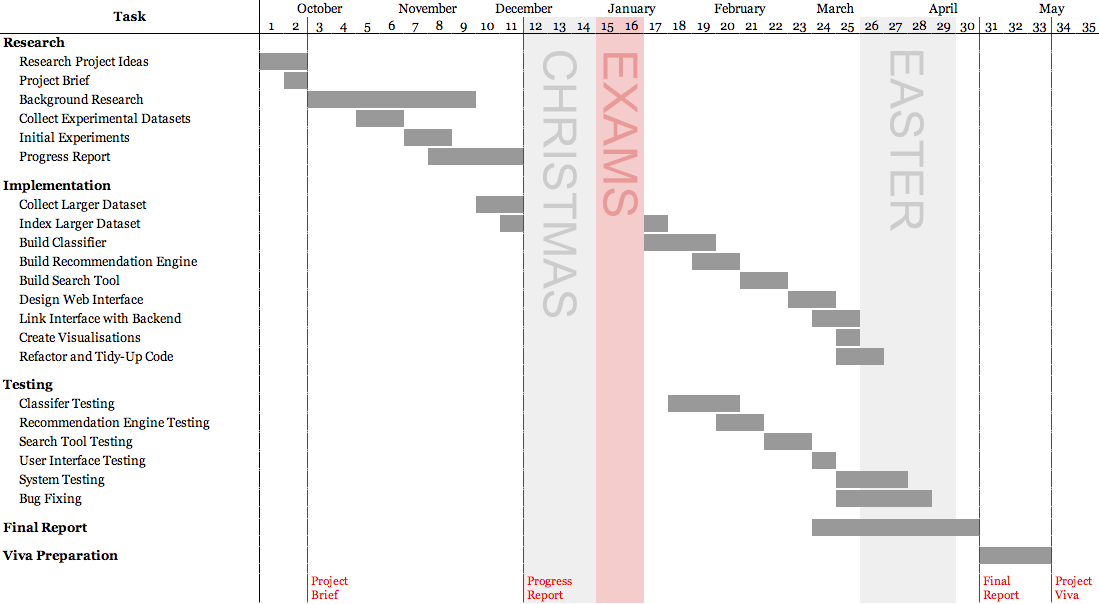
\includegraphics[height=0.86\textwidth]{gantt.png}
        \caption*{A Gantt chart showing the \emph{scheduled} progression through the different aspects of the project.}
    \end{figure}

    \begin{figure}[H]
        \centering
        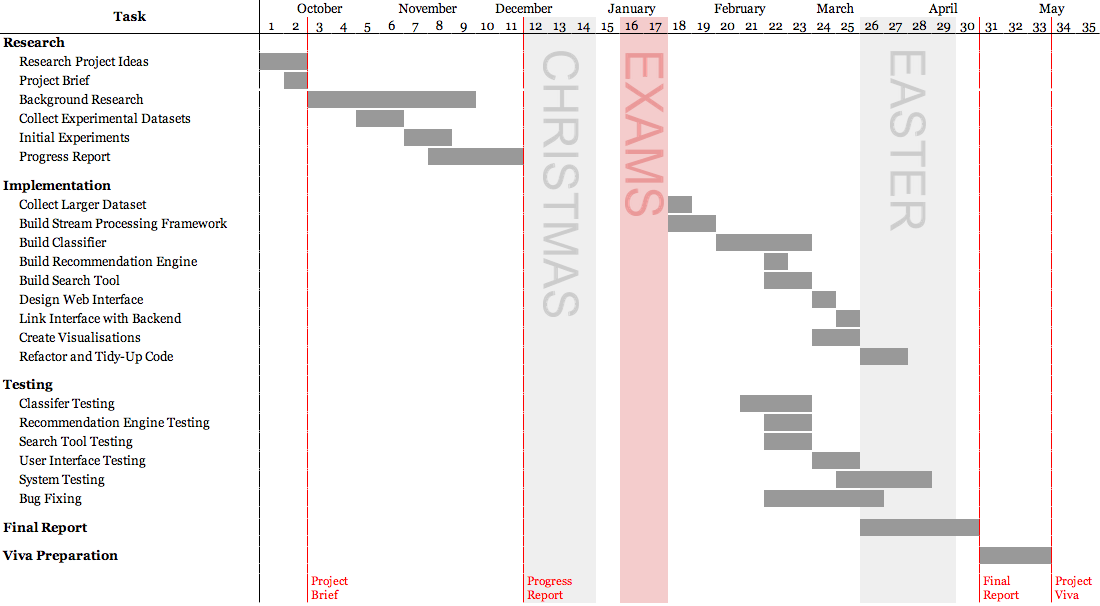
\includegraphics[height=0.86\textwidth]{gantt-actual.png}
        \caption*{A Gantt chart showing the \emph{actual} progression through the different aspects of the project.}
    \end{figure}
\end{landscape}
\pagebreak

\section{Project Directory Listing}
\label{appendix:directorytree}
\todo[inline]{Add directory tree}
\pagebreak

\section{Original Project Brief}
\begin{center}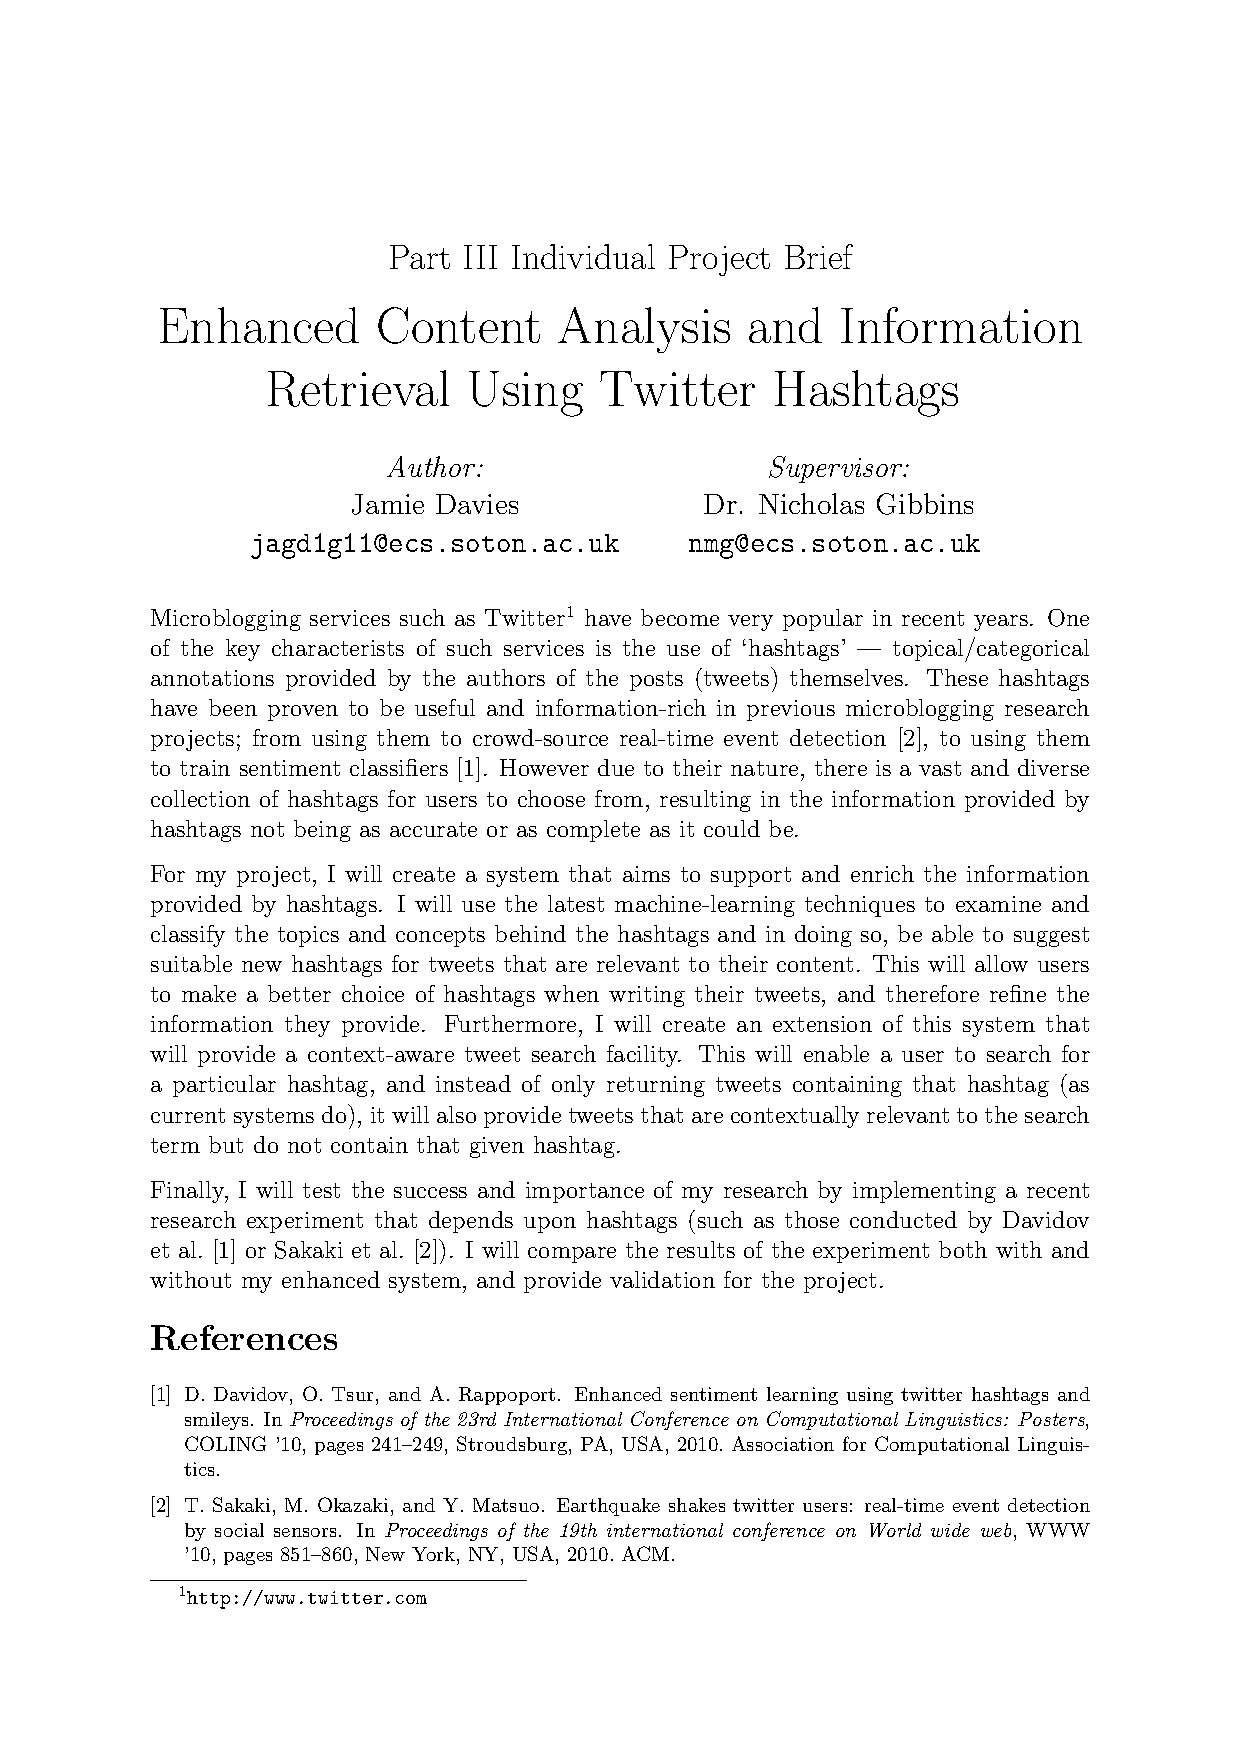
\includegraphics[trim=2.5cm 2.5cm 2.5cm 3.5cm,clip,width=\textwidth]{../brief/brief.pdf}\end{center}
\end{subappendices}

\end{document}
